\documentclass[12pt]{report}
\usepackage{fancyhdr}
\usepackage{amsmath}
\usepackage{amsfonts}
\usepackage{color}
\usepackage{latexsym}
\usepackage{amssymb}
\usepackage{amsthm}
\usepackage{graphicx}
\usepackage{enumerate}
\usepackage{mflogo}
\usepackage{tikz}
 \usetikzlibrary{calc} 
\usepackage{float}


\newtheorem{theorem}{Theorem}
\newtheorem{definition}{Definition}
\newtheorem{problem}{Problem}
\newtheorem{remarks}{Remarks}
\newtheorem{proposition}{Proposition}
\newtheorem{conjecture}{Conjecture}
\newtheorem{lemma}{Lemma}
\newtheorem{step}{Step}
\newtheorem{case}{Case}
\newtheorem{corollary}{Corollary}




\author{Gao Mou\thanks{Nanyang Technological University. Email: gaom0002@e.ntu.edu.sg}}
\title{The $k$-walks in 2$K_2$-free graphs}
\begin{document}
\pagenumbering{roman}
\begin{titlepage}




\maketitle



A thesis submitted to the Nanyang Technological University in fulfilment of the requirement for the degree of Doctoral of Philosophy of Mathematics
\end{titlepage}

\listoffigures

\tableofcontents

\begin{abstract}
In this thesis, we first review the progress, old or recent, on the research area of Hamiltonicity.

In addition, we talk about several generalizations of Hamilton cycles, i.e. $k$-walks, $k$-trees, Hamilton-prisms and edge-dominating cycles. And we also investigate the relation between them. Especially, we focus on the Jackson-Wormald Conjecture and show that if a graph has an edge-dominating cycle, then Jackson-Wormald conjecture holds for this graph.

The central task of this thesis is to prove that Jackson-Wormald conjecture is true for $2K_2$-free graphs. The key part is to prove that if a $2K_2$-free graph is not a tree, then it admits an edge-dominating cycle. Theoretically, this is a corollary of a result by Veldman \cite{veldman1983existence}, however, we provide an efficient algorithm to find the edge-dominating cycle, and thus find the $k$-walk. 

Another main result of this thesis is to prove that every $(1+\epsilon)$-tough $2K_2$-free graph is prism-Hamiltonian. Generally, being prism-Hamiltonian is a stronger property than admitting $k$-walks for all $k\ge2$, but weaker than being traceable.

Finally, we list several results on the existence of 2-walk under the assumption of 1-tough for some other graphs. And also pose some conjectures for further research.
\end{abstract}

\chapter{Preliminary}\label{cpre}
\pagenumbering{arabic}

In this thesis, we make a summary on the recent progression in the area of hamiltonicity and $k$-walks of some special kinds of graphs under some toughness conditions. Additionally, we introduce  Jackson-Wormald Conjecture and prove that it is true for $2K_2$-free graphs.

In Chapter \ref{cpre}, we introduce some elementary notions and definitions in graph theory. In Chapter \ref{c2ht}, we talk about the concept of toughness and its many applications in graph theory. In Chapter \ref{ch3edcah}, we discuss a generalization of Hamilton cycles, edge-dominating cycles. And we also have a look at an important application of edge-dominating cycles on the research of line graphs. Next, in Chapter \ref{ch4kw}, we introduce some other generalizations of Hamilton cycles, $k$-walks and Hamilton prisms, and then we show the first main result of this thesis: for the graphs containing edge-dominating cycles, a conjecture by Jackson and Wormald is true. In Chapter \ref{chap2k2fg}, we prove another main result that for any $\frac{1}{k-1}$-tough $2K_2$-free graph $G$, there is a $k$-walk, and it can be found in time polynomial to the number of vertices $|V(G)|$. What is more, we also prove that every $(1+\epsilon)$-tough $2K_2$-free graphs is prism-Hamiltonian.

\section{Definitions and terminologies}
The field of graph theory is considered to begin from a paper \cite{euler1741solutio} by the Swiss mathematician Leonhard Euler, one of the most excellent mathematicians ever in the history, in 1736. In the 1700s, the Pregolya River passed through a city named Konigsberg in the East Prussian, where seven bridges were built across this river. The residents in the city enjoyed strolling these seven bridges, however, as hard as they tried, nobody of them was ever able to walk a route that crossed each of these bridges exactly once. Euler noticed on this interesting phenomenon, and did a research on that. Then, the subject graph theory began.



Most definitions and terminologies in this thesis follow \cite{harris2008combinatorics}, \cite{bomu08} and \cite{diestel2000graph}, so we strongly recommend readers look at these three books for more details.
\subsection{Graphs}
A {\em graph} is a pair $G=(V,E)$ of sets satisfying $E\subset[V]^2$, so the elements of $E$ are 2-element subset of $V$. All the graphs talked in this thesis are finite graphs, i.e. for any graph $G=(V,E)$, we assume both $|V|$ and $|E|$ are finite. A graph with vertex set $V$ is said to be a graph on $V$. The vertex set of a graph is denoted as $V(G)$, its edge set as $E(G)$.
For two graphs $G=(V,E)$ and $G'=(V',E')$, if $V'\subset V$ and $E'\subset E$, then we say $G'$ is a subgraph of $G$, written as $G'\subset G$. 
If $G'\subset G$ and $G'$ contains all the edges $xy\in E$ with $x,y\in V'$, then $G'$ is called an {\em induced subgraph} of $G$. What is more, if $U\subset V$ is any subset of vertices, then $G|_U$ stands for the graph on $U$ whose edges are precisely the edges of $G$ with both ends in $U$. And we say $G'\subset G$ is a spanning subgraph of $G$ if $V'=V$.

For any $v\in V(G)$, $N_G(v)$ (or briefly $N(v)$) denotes the set of neighbors of $v$ in $G$. Additionally, the neighborhood of a subset $S$ of vertices is denoted as $N(S)=\cup_{v\in S}N(v)$.
The {\em degree} $d_G(v)=d(v)$ of a vertex $v$ is the number of edges incident to $v$, this is equal to the number of neighbours of $v$ when $G$ is a simple graph, who does not allow multiple edges.
A vertex of degree 0 is called an {\em isolated} vertex. A vertex of degree 1 is called a {\em suspended} vertex. The minimum degree of a graph $G$ is denoted by $\delta(G)=\min\{d(v)|v\in V(G)\}$. The maximum degree of a graph $G$ is denoted by $\Delta(G)=\max\{d(v)|v\in V(G)\}$.
Obviously, we have the following observation:
\begin{proposition}
The number of vertices of odd degree in a graph is always even.
\end{proposition}
Let $c(G)$ denote the length of a longest cycle in $G$, namely {\em circumference}.
If all the vertices of $G$ are pairwise adjacent, then $G$ is {\em complete}. A complete graph on $n$ vertices is denoted as $K_n$.
The greatest integer $r$ such that $K_r\subset G$ is the {\em clique number} $\omega(G)$ of $G$. 




A multigraph is a graph which possibly has loops and multiple edges.
For an integer $m$, $m*G$ stands for the multigraph obtained from $G$ by taking each edge $m$ times.

In a graph $G$, a subset of vertices (or the induced subgraph on this subset) $S\subset V(G)$ is called {\em dominating}, if $S^{\perp}:=S\cup N(S)=V(G)$. 
$S$ is called {\em edge-dominating}, if the induced subgraph on $V(G)-S$ has no edge, i.e. each edge $e\in E(G)$ has at least one endpoint in $S$.
$S$ is called {\em weakly-dominating}, if any edge $e\in E(G)$ has at least one endpoint adjacent to some vertices in $S$.


\subsection{Paths, trails and walks}

A {\em walk} (of length $k$) in a graph $G$ is a non-empty alternating sequence $v_0e_0v_1e_1\ldots e_{k-1}v_k$ of vertices and edges in $G$ such that $e_i=v_iv_{i+1}$ for all $i<k$. If $v_0=v_k$, the walk is said to be {\em closed}. A {\em path} is a walk with all vertices distinct. 
\begin{proposition}
Every walk between two distinct vertices contains a path between these vertices.
\end{proposition}

The following theorem is one of the cornerstones of graph theory.
\begin{theorem}[Menger 1927]\label{mengert27}
For a graph $G$, assume $A,~B\subset V(G)$. Then the minimum number of vertices separating $A$ from $B$ in $G$ is equal to the maximum number of disjoint $A$-$B$ paths in $G$.
\end{theorem}




A graph $G$ is called {\em connected} if any two of its vertices are linked by a path in $G$. A maximal connected subgraph of $G$ is called a {\em component} of $G$.  For a (non-connected) graph $G$, the number of components is usually denoted by $\Omega(G)$.
$G$ is called {\em $k$-connected} if $|G|>k$ and $G-X$ is connected for every set $X\subset V(G)$ with $|X|<k$. The greatest integer $k$ such that $G$ is $k$-connected is the {\em connectivity} $\kappa(G)$ of $G$.



A {\em trail} is a walk that does not repeat any edge.
A closed trail is called a {\em circuit}. A cycle is a circuit which does not repeat any vertex.


If a trail in a graph $G$ includes every edge of $G$, then that trail is said to be an {\em Eulerian trail}. Similarly, an {\em Eulerian circuit} in a graph is a circuit includes every edge of the graph. What is more, a graph containing an Eulerian circuit is called an {\em Eulerian graph}.

It is well known that:
\begin{theorem}[Euler 1736]
For a connected graph $G$, it is an Eulerian graph if and only if evry vertex in $G$ has even degree.
\end{theorem}



\subsection{Bipartites and matchings}

Let $r\ge2$ be an integer. A graph $G=(V,E)$ is called $r$-partite if $V$ admits a partition into $r$ classes such that every edge has its ends in different classes, i.e. vertices in the same partition class must not be adjacent. Additionally,``2-partite" is usually called {\em bipartite} for convenience.
\begin{proposition}\label{bipoefpro3}
A graph is bipartite if and only if it contains no odd cycle.
\end{proposition}

A set $M$ of independent edges in a graph $G=(V,E)$ is called a {\em matching}. 
$M$ is a matching of $U\subset V$ if every vertex in $U$ is incident with an edge in $M$.
Let $G=(V,E)$ be a bipartite with partition $\{A,B\}$. Then we have the following famous theorem to decide whether there is a matching in $G$ for $A$. Although almost every textbook on graph theory contains a proof of Hall' Theorem, but we still include it to be self-contained, since Hall' Theorem, and its variations are very important in the proof of our main results.
\begin{theorem}[Hall 1935]\label{hallori1th}
$G$ contains a matching of $A$ if and only if $|N(S)|\ge|S|$ for all $S\subset A$.
\end{theorem}
\begin{proof}
Obviously, the direction ``$\Rightarrow$" is trivial.

To prove the direction ``$\Leftarrow$", we use mathematical induction on the size of $A$.
If $|A|\le1$, there is nothing to prove.
Suppose that for any $S\subset A$, with $S\neq\emptyset,~A$, we have $|N(S)|>|S|$. Then take any $xy\in E(G)$ (where $x\in A$). So $G-x$ satisfies Hall's condition. By the induction hypothesis, the induced subgraph $G-\{x,y\}$ contains a matching. Thus $G$ contains a matching.

Otherwise, there is a critical set $T\subset A$, $T\neq\emptyset,~A$ with $|N(T)|=|T|$. Now, let $G_1$ be the induced subgraph of $G$ on the vertex set $T\cup N(T)$, and $G_2$ be the induced subgraph of $G$ on the vertex set $(A-T)\cup(B-N(T))$. Obviously, both $G_1$ and $G_2$ satisfy Hall's condition. Then by induction hypothesis, there is a matching on $G_1$ and $G_2$, giveing a matching on $G$.


\end{proof}


This theorem can be generalized as follow:
\begin{theorem}[Polygamous form of Hall' Theorem]
Let $d\ge1$ be an integer. If $|N(S)|\ge d|S|$ for all subset $S\subset A$, then we can match each $a\in A$ to $d$ elements of $B$, the different $d$-element sets being disjoint.
\end{theorem}
\begin{proof}

Replace each $x\in A$ with $d$ nodes adjacent to $N(x)$, Hall's Theorem gives a matching.

\end{proof}


What is more, we can even remove the requirement of $d\ge1$, to obtain the following generalization.
\begin{theorem}\label{zuiqianghallt}
Let $p\ge1$ be an integer. If $|N(S)|\ge\frac{|S|}{p}$ for all subset $S\subset A$, then we can find a subset of the edge set $E'\subset E(G)$ such that each vertex $v\in A$ is incident to exactly one edge $e\in E'$ and each vertex $u\in B$ is incident to at most $p$ edges in $E'$.
\end{theorem}





\subsection{$k$-factors}


For any graph $G$, if all the vertices of $G$ have the same degree $k$, then $G$ is {\em $k$-regular}, or simply {\em regular}. Especially, a 3-regular graph is called {\em cubic}.
\begin{definition}
A $k$-regular spanning subgraph is called a $k$-factor.
\end{definition}
Clearly, a subgraph $H\subset G$ is a 1-factor of $G$ if and only if $E(H)$ is a matching of $V(G)$. Additionally, $H\subset G$ is a 2-factor if and only if $H$ is a union of independent cycles spanning $V(G)$.

We strongly recommend the readers who are interested in this topic to consult an excellent survey \cite{plummer2007graph}. In this thesis, we only list some important results relevant to our main topic.


The following proposition can be considered as a corollary of Theorem \ref{hallori1th}.

\begin{proposition}\label{propkrto1f}
If bipartite $G$, with two parts $A$ and $B$, is $k$-regular for some $k\ge1$, then $G$ has a 1-factor.
\end{proposition}
\begin{proof}
Becasue $G$ is $k$-regular, clearly, $|A|=|B|$. Obviously, any set $S\subset A$ is jointed to $N(S)$ by totally $k|S|$ edges, and these are among the $k|N(S)|$ edges in $G$ incident with $N(S)$. Thus $k|S|\le k|N(S)|$, so by Theorem \ref{hallori1th}, $G$ has a matching.




\end{proof}


It is widely believed that Hall' Theorem is one of the most frequently applied theorems in graph theory. Usually, however, recasting a problem in the setting of bipartite matching requires some technical adaptation. For example, we now use Hall' Theorem to drive one of the earliest results in graph theory. This concise proof comes from \cite{diestel2000graph}.

\begin{theorem}[Peterson 1891]\label{petkre2fac}
For any integer $k\ge1$, every $2k$-regular graph has a 2-factor.
\end{theorem}

\begin{proof}
Without loss of generality, we can assume $2k$-regular graph $G$ is connected. Obviously, $G$ contains an Euler tour, say $v_0e_0\ldots e_{l-1}v_l$ with $v_0=v_l$. We replace every vertex $v$ by a pair $(v^-,v^+)$, and every $e_i=v_iv_{i+1}$ by the edge $v_i^+v^-_{i+1}$. The resulting graph $G'$ is clearly a $k$-regular bipartite. By Proposition \ref{propkrto1f}, it has a 1-factor. Now, collapsing every vertex pair $(v^-,v^+)$ back into a single vertex $v$, we turn this factor of $G'$ into a 2-factor in $G$.
\end{proof}

The following famous theorem provides a necessary and sufficient condition for the existence of 1-factor.
\begin{theorem}[Tutte 1947]\label{tutte otto1f}
A graph $G$ contains a 1-factor if and only if $\Omega_O(G-S)$, the number of odd components in $G-S$, satisfies $\Omega_O(G-S)\le|S|$ for all $S\subset V(G)$.
\end{theorem}


What is more, Tutte also gave us a more generalized criterion for a graph to have a $k$-factor \cite{tutte1952factors}.

\begin{theorem}[Tutte 1952]\label{tut1952cri1}
For any subsets $S,~T\subset V(G)$, let $e_G(S,T)$ denote the number of edges joining $S$ and $T$. And for any disjoint subsets $A,~B\subset V(G)$, let $h_G(A,B)$ be the number of connected components $C$ of $G-(A\cup B)$ satisfying $k|C|+e_G(C,B)\equiv1(\mod2)$. Define $\delta_{G,k}(A,B)=k|A|+\sum_{x\in B}d_{G-A}(x)-k|B|-h_G(A,B)$. Then we have:
\begin{enumerate}
\item $\delta_{G,k}(A,B)\equiv k|V(G)|(\mod2)$.
\item A graph $G$ has a $k$-factor if and only if $\delta_{G,k}(A,B)\ge0$ for any disjoint subsets $A,~B\subset V(G)$.
\end{enumerate}
\end{theorem}



\begin{definition}
An edge $e$ in a connected graph $G$ is called a bridge, if the graph $G'$, obtained by deleting $e$ from $G$, is no longer connected.
\end{definition}
\begin{definition}\label{bilede}
A graph $G$ is called bridgeless if $G$ does not contain bridges.
\end{definition}
Then we have the following corollary of Theorem \ref{tutte otto1f}

\begin{theorem}[Petersen 1891]\label{petbrile1fa}
Every bridgeless cubic graph contains a 1-factor.
\end{theorem}
\begin{proof}
For any $S\subset V(G)$, consider an odd component $C$ of $G-S$. Because $G$ is cubic, the degrees (in $G$) of the vertices in $C$ sum to an odd number, but only an even part of this sum arises from edges of $C$. Thus $G$ has an odd number of edges between $S$ and $C$. And therefore there are at least 3 such edges, since $G$ has no bridge. The total number of edges between $S$ and $G-S$ is therefore at least $3\Omega_O(G-S)$. But it is at most $3|S|$, since $G$ is cubic. So, we get $\Omega_O(G-S)\le|S|$. Then by Theorem \ref{tutte otto1f}, $G$ has a 1-factor.
\end{proof}


\section{Planar graphs}\label{secnoplg}
A graph is called {\em planar} if it can be drawn in the plane in such a way that pairs of edges intersect only at vertices, if at all. A drawing of a planar graph $G$ in the plane in which edges intersect only at vertices is called a {\em planar representation} of $G$.
Given a planar representation of $G$, a {\em region} is a maximal section of the plane in which any two points can be joint by a curve that does not intersect any part of $G$.

Euler discovered a relationship between the number of vertices, edges and regions of a graph.
\begin{theorem}[Euler 1758]
If  $G$ is a connected planar graph with $n$ vertices, $q$ edges and $r$ regions, then $n-q+r=2$.
\end{theorem}

Let $e=xy$ be an edge of a graph $G=(V,E)$. And let $G/e$ denote the graph obtained from $G$ by {\em contracting} the edge $e$ into a new vertex $v_e$, which becomes adjacent to all the former neighbors of $x$ and $y$ in $G$, i.e. $G/e$ is a graph $(V',E')$ with vertex set $V'=(V-\{x,y\})\cup\{v_e\}$ and edge set $E'=\{vw\in E:\{v,w\}\cap\{x,y\}=\Phi\}\cup\{v_ew:xw\in E-\{e\}~or~yw\in E-\{e\}\}$.

More generally, if $G=(V(G),E(G))$ is a graph and $X=(V(X),E(X))$ is another graph, and $\{V_x:x\in V(X)\}$ is a partition of $V(G)$ into connected subsets such that, for any two vertices $x,y\in V(X)$, there is a $V_x-V_y$ edge in $G$ if and only if $xy\in E(X)$, we call the sets $V_x$ are the {\em branch sets} of $G$. Intuitively, we obtain $X$ from $G$ by contracting every branch set into a single vertex and deleting all parallel edges and loops that may arise. 

We call $X$ a {\em minor} of $Y$, denoting as $X\preccurlyeq Y$, if $X$ can be obtained from a subgraph $Y'\subset Y$ by a sequence of contracting. 

If a graph $G$ is obtained by replacing the edges of $X$ with independent paths between their ends, then we call $G$ a {\em subdivision} of $X$. If a subdivision $H$ of $X$ is a subgraph of $Y$, we say that $X$ is a {\em topological minor} of $Y$.

We have the following famous theorem on planar graphs:
\begin{theorem}[Kuratowski 1930]\label{plgfodmthmku}
The following assertions are equivalent for a graph $G$:
\begin{enumerate}
\item $G$ is planar;
\item $G$ has neither $K_5$ nor $K_{3,3}$ as a minor;
\item $G$ has neither $K_5$ nor $K_{3,3}$ as a topological minor.
\end{enumerate}
\end{theorem}




\section{Chordal graphs}

Now, let us look at a family of graphs which will be mentioned several times throughout this thesis, the chordal graphs.

\begin{definition}\label{defchor}
A graph is $k$-chordal if any longest chordless cycle in $G$ has length at most $k$. 3-chordal graphs are called chordal graphs for short.
\end{definition}
That means a graph $G$ is {\em chordal} if it contains no induced cycles of length at least 4.

We have the following description of chordal graphs.

A vertex $x$ of a graph $G$ is called a {\em simplicial vertex} of $G$, if the subgraph of $G$ induced by the neighbirs of $x$ is complete.
The following property of chordal graphs comes from \cite{dirac1961rigid}.
\begin{proposition}[Dirac 1961]\label{pdir61}
Every chordal graph has a simplicial vertex.
\end{proposition}

An ordering $x_1x_2\cdots x_n$ of the vertex set of a graph $G$ is said to be a {\em perfect elimination order}, if $x_1$ is a simplicial vertex of $G$ and $x_i$ is a simplicial vertex of $G-\{x_1,\ldots,x_{n-1}\}$ for $i=2,\ldots,n$. Then we have:
\begin{proposition}\label{c2.2}
A graph is chordal if and only if it has a perfect elimination order.
\end{proposition}
\begin{proposition}\label{c2.3}
Let $G$ be an $l$-connected chordal graph, $x_1x_2\cdots x_n$ be a perfect elimination order of $G$, and $i\in\{1,\ldots,n-1\}$. Then the graph $G-\{x_1,\ldots,x_i\}$ is either $l$-connected or complete.
\end{proposition}


For the readers who are interested in the topic chordal graphs, we strongly recommend them to consult \cite{bauer2000chordality}, \cite{bauer2000not}, \cite{bohme1999more} and \cite{chen1998tough} for more details.












\chapter{Hamiltonicity and toughness}\label{c2ht}
In this chapter, we first make a concise review on the development and history of the research on Hamiltonicity. Additionally, we shall  focus on the relation between the concept of toughness and the existence of Hamilton cycle, i.e. the Chv{\'a}val's Conjecture. We shall both  make a general introduction and list several concrete examples, positive or negative, on the research of this conjecture.

\section{Hamilton graphs}

The story of Hamilton graphs can be traced back to 1850's. In 1859, the English game company Jaques and Son bought the right to manufacture and sell a game, named "The Icosian Game", from the prominent mathematician Sir William Rowan Hamilton. And the problem of finding a Hamilton cycle came up here. From that time, this topic is one of the central and fundamental problems in graph theory. We strongly recommend readers to consult \cite{gould1991updating} and \cite{MR2221006} for a detailed history of this topic.

If a path $P$ spans all the vertices of $G$, i.e. $V(P)=V(G)$, then $P$ is said to be a {\em Hamilton path} of $G$. Any graph contains a Hamilton path is called {\em traceable}. If a cycle $C$ spans the vertices of a graph $G$, such a cycle is called {\em Hamilton cycle}, and a graph containing a Hamilton cycle is called a Hamilton graph.

The following result may be considered as one of the earliest one on this topic.

\begin{theorem}[Dirac 1952]\label{dirac1952th}
Every graph with $n\ge3$ vertices and minimum degree at least $n/2$ has a Hamilton cycle
\end{theorem}


In 1960, Ore generalized Dirac's results to the following form:
\begin{theorem}[Ore 1960]\label{ore1960hth1}
If $G$ is a graph of order $n$ such that $d(x)+d(y)\ge n$ for every pair of nonadjacent vertices $x,y\in V(G)$, then $G$ is Hamiltonian.
\end{theorem}

In \cite{bondy1976a}, Bondy and Chv{\'a}tal extended Ore's Theorem. Define the {\em k-closure} of $G$, $C_k(G)$, as the graph obtained by recursively joining pairs of nonadjacent vertices whose degree sum is at least $k$, until no such pair remains. Then we have:
\begin{theorem}[Bondy and Chv{\'a}tal 1976]\label{thmcloham1}
A graph $G$ of order $n$ is Hamiltonian if and only if $C_n(G)$ is Hamiltonian.
\end{theorem}

Let $\alpha(G)$ denote the {\em independence number}, the maximal size of independent set, of $G$. It is interesting that the combination of high connectivity and low independence number produce a sufficient condition for Hamiltonicity. In \cite{chvatal1972a}, Chv{\'a}tal and Erd{\"o}s proved that
\begin{theorem}[Chv{\'a}tal and Erd{\"o}s 1972]\label{kageaptohathe}
Every graph $G$ with $|V(G)|\ge3$ and $\kappa(G)\ge\alpha(G)$ is Hamiltonian.
\end{theorem}
In the same paper, they also proved:
\begin{theorem}[Chv{\'a}tal and Erd{\"o}s 1972]\label{thmce15}
Every graph $G$ with $|V(G)|\ge3$ and $\kappa(G)\ge\alpha(G)-1$ admits a Hamilton path.
\end{theorem}

For planar graph, there is a concise and beautiful result.

\begin{theorem}[Tutte 1956]\label{thm4cpgih1}
Every 4-connected planar graph is Hamiltonian.
\end{theorem}
We will mention this theorem again in the next chapter.

If $G$ is a graph with $n$ vertices and their degrees $d_1\le\ldots\le d_n$, then the $n$-tuple $(d_1,\ldots,d_n)$ is called the {\em degree sequence} of $G$.
\begin{theorem}[Chv{\'a}tal 1972]
A graph $G$ with degree sequence $(d_1,\ldots,d_n)$, $n\ge3$, is Hamiltonian if and only if the following holds for every $i<n/2$:
$$d_i\le i\Rightarrow d_{n-i}\ge n-i.$$
\end{theorem}





\section{Toughness and Chv{\'a}tal's Conjecture}
In 1973, Chv{\'a}tal \cite{chvatal1973tough} introduced the concept of toughness. After that, problems about this concept become a central part in the research of Hamiltonicity of graphs. And from that time, a lot of research has been done, most of the research was on the toughness conditions to the existence of cycle structure. Additionally, the most challenging problem is still unsolved: 
\begin{conjecture}[Chv{\'a}tal]\label{cj1chath}
There is a finite constant $t$ such that every $t$-tough graph is Hamiltonian.
\end{conjecture}
And we strongly recommend readers to consult an excellent survey \cite{MR2221006} on this topic for more detailed information.

\begin{definition}[Chv{\'a}tal 1973]\label{c1}
Let $G$ be a graph and $t$ a real number such that the implication $k(G-S)>1\Rightarrow |S|\ge t\cdot k(G-S)$ holds for each set $S$ of points of $G$. Then $G$ will be said to be $t$-tough. Here $k(G-S)$ denotes the number of components in the graph $G-S$.
\end{definition}
That is, $G$ is {\em $t$-tough} if $G$ cannot be split into $m$ (with $m>1$) components by removing less than $mt$ vertices.
Obviously, a $t$-tough graph is $s$-tough for all $s<t$. If $G$ is not complete, then there is a largest $t$ such that $G$ is $t$-tough; this maximal $t$ will be called the {\em toughness} of $G$ and denoted by $t(G)$. On the other hand, a complete graph contains no point-cutset and so it is $t$-tough for every $t$. Thus, we set $t(K_n)=+\infty$ for every $n$. Then we can write $t(G)=\min|S|/k(G-S)$, where $S$ ranges over all point-cutsets of $G$.

The following observation is both obvious and important.
\begin{proposition}\label{prokg2t}
For the toughness $t(G)$ and connectivity $\kappa(G)$ of any graph $G$, we have $\kappa(G)\ge2t(G)$.
\end{proposition}





Here we list several important results in the history on this topic.
\begin{theorem}[Jung 1987]
Let $G$ be a 1-tough graph on at least 11 vertices, and for any pair of nonadjacent vertices $x,y\in V(G)$, $d(x)+d(y)\ge n-4$. Then $G$ is Hamiltonian.
\end{theorem}


\begin{theorem}[Bauer, Chen and Lasser 1991]
Let $G$ be a $(1+\epsilon)$-tough graph (with any $\epsilon>0$) on at least 30 vertices, and for any pair of nonadjacent vertices $x,y\in V(G)$, $d(x)+d(y)\ge n-7$. Then $G$ is Hamiltonian.
\end{theorem}

\begin{theorem}[Bauer, Broersma, van den Heuvel and Veldman 1995]
Let $G$ be a $t$-tough graph on $n\ge3$ vertices with the minimal degree $\delta>n/(t+1)-1$. Then $G$ is Hamiltonian.
\end{theorem}

\begin{theorem}[Jung, Wittmann 1999]
Let $G$ be a 2-connected $t$-tough graph on $n$ vertices. Then $c(G)\ge\min\{n,(t+1)\delta+t\}$.
\end{theorem}

Conjecture \ref{c1} was believed to be true with $t=2$, until the year 2000, Bauer, Broersma and Veldman \cite{bauer2000not} provided a construction of $(9/4-\epsilon)$-tough graphs that are not Hamiltonian, for every $\epsilon>0$. More exactly, that is:
\begin{theorem}[Bauer, Broersma and Veldman 2000]\label{exa2000nh}
For every $\epsilon>0$, there is a $(9/4-\epsilon)$-tough  graph containing no Hamilton path.
\end{theorem}

\begin{proof}
The proof is contructive. For any graph $H$ and its two vertices $x$ and $y$, let us define a graph $G(H,x,y,l,m)$ in the following way. Take $m$ disjoint copies of $H$, say $H_1,\ldots,H_m$, with $x_i$ and $y_i$ the vertices in $H_i$ corresponding to the vertices $x$ and $y$. Let $F_m$ stand for the graph obtained from $H_1\cup\cdots H_m$ by adding all possible edges between $\{x_1,\ldots,x_m,y_1,\ldots,y_m\}$. Denote $T=K_l$, the complete graph on $l$ vertices. Let $G(H,x,y,l,m)$ be the join $T\lor F_m$. Now, suppose $H$ is a graph, where $x$ and $y$ cannot be connected by any Hamilton path in $H$, and assume $m\ge2l+3$. Then we claim that $G(H,x,y,l,m)$ does not admit any Hamilton path.

Otherwise, assume $G(H,x,y,l,m)$ admits a Hamilton path, say $P$. Then, the intersection of $F_m$ and $P$ consists of a collection of no more than $l+1$ disjoint paths, denoted by $\mathcal{P}$. They together contain all the vertices of $F_m$. As the assumption, $m\ge2(l+1)+1$, there exists a subgraph $H_{i_0}$ in $F_m$ such that no endvertex of any path of $\mathcal{P}$ lies in $H_{i_0}$. Therefore the intersection of $P$ and $H_{i_0}$ is a path with endpoint $x_{i_0}$ and $y_{i_0}$ that contains all vertices of $H_{i_0}$. This contradicts with the assumption that $H_{i_0}$ is a copy of the graph $H$ containing no Hamilton path connecting $x$ and $y$.

Now, suppose $L$ is the following graph (Figure \ref{2sqr}).
\begin{figure}[h]
\begin{center}

\setlength{\unitlength}{1mm}
\begin{picture}(60,60)
\put(10,30){\circle*{2}}
\put(20,20){\circle*{2}}
\put(20,40){\circle*{2}}
\put(30,10){\circle*{2}}
\put(30,50){\circle*{2}}
\put(40,20){\circle*{2}}
\put(40,40){\circle*{2}}
\put(50,30){\circle*{2}}
\put(10,30){\line(1,1){20}}
\put(30,10){\line(1,1){20}}
\put(10,30){\line(1,-1){20}}
\put(30,50){\line(1,-1){20}}
\put(20,20){\line(1,0){20}}
\put(20,20){\line(0,1){20}}
\put(20,40){\line(1,0){20}}
\put(40,20){\line(0,1){20}}
\put(6,30){u}
\put(52,30){v}

\end{picture}

\end{center}

\caption{}\label{2sqr}
\end{figure}
\newpage

Now, we claim that for any integers $l\ge2$ and $m\ge1$, we have
$$t(G(L,u,v,l,m))=\frac{l+4m}{2m+1}.$$
Choose $S\subset V(G)$ such that $\Omega(G-S)>1$ and $t(G)=\frac{|S|}{\Omega(G-S)}$. Clearly, $V(T)\subset S$. Now, denote $S_i=S\cap V(L_i)$ and $s_i=|S_i|$, and let $\Omega_i$ stand for the number of components of $L_i-S_i$ that contain neither $v_i$ nor $u_i$. Then we have:
$$t(G)=\frac{l+\sum^m_{i=1}s_i}{c+\sum^m_{i=1}\Omega_i}\ge\frac{l+\sum^m_{i=1}s_i}{1+\sum^m_{i=1}\Omega_i},$$
in which $c=0$ if $u_i,v_i\in S_i$ for all $i\in\{1,\ldots,m\}$, and 1 if otherwise.

Here we need to show $s_i\ge2\Omega_i$, for $i=1,\ldots,m$.

First, because $L-\{u,v\}$ has independence number 2, then $\Omega_i\le2$. Obviously, $s_i\ge2\Omega_i$ when $\Omega_i=0$ or $\Omega_i=1$. and we can also check that $s_i\ge2\Omega_i$ if $\Omega_i=2$. Then we get $$t(G)\ge\frac{l+2\sum^m_{i=1}\Omega_i}{1+\sum^m_{i=1}\Omega_i}.$$

When $l\ge2$, the lower bound for $t(G)$ is a nonincreasing function about $\sum^m_{i=1}\Omega_i$, so it is minimized when $\Omega_i=2$ for all $i=1,\ldots,m$. Therefore $t(G)\ge\frac{l+4m}{2m+1}$.

Denote $U=V(T)\cup U_1\cdots U_m$, where $U_i$ is the set of vertices of $L_i$ with degree 4 in $L_i$. And we have $t\le\frac{|U|}{\Omega(G-U)}=\frac{l+4m}{2m+1}$.

Finally, since $L$ contains no Hamilton path connecting $u$ and $v$, so the graph $G(L,u,v,l,2l+3)$ has no Hamilton path for any $l$. And it has toughness $\frac{9l+12}{4l+7}$ for all $l\ge2$.


\end{proof}





\section{Toughness and $k$-factors}

Recall that a 2-factor is a generalization of a Hamilton cycle. As we pay much attention to the relation between the toughness of graphs and the existence of Hamilton cycle, it is reasonable to ask what is the relation between the toughness of graphs and the existence of 2-factors or $k$-factors.


\subsection{The existence of $k$-factors}
Around 30 years ago, Enomoto, Jackson, Katerinis and Saito (see \cite{enomoto1985toughness},\cite{enomoto1986toughness}) proved that if a $k$-tough graph satisfies some trivial conditions, then it contains a $k$-factor.

Specifically, they proved:

\begin{theorem}[Enomoto, Jackson, Katerinis and Saito 1985]\label{kttokf19851}
Suppose $|V(G)|\ge k+1$ and $k|V(G)|$ even, if for all $S\subset V(G)$, such that $\Omega(G-S)>1$ we have $|S|\ge k\Omega(G-S)-\frac{7}{8}k$, then $G$ contains a $k$-factor.
\end{theorem}

Obviously, we have:
\begin{corollary}
For any $k$-tough graph $G$, if $|V(G)|\ge k+1$ and $k|V(G)|$ is even, then $G$ contains a $k$-factor.
\end{corollary}

More specifically, when $k=2$, we have:

\begin{corollary}\label{kttokfejks}
Every 2-tough graph on at least 3 vertices contains a 2-factor.
\end{corollary}




\subsubsection{Two lemmas}
Recall the definitions and notions in Theorem \ref{tut1952cri1}, that $$\delta_{G,k}(A,B)=k|A|+\sum_{x\in B}d_{G-A}(x)-k|B|-h_G(A,B),$$ where $A$ and $B$ are two disjoint subsets of $V(G)$.
The following two lemmas are the key points in the proof of Theorem \ref{kttokf19851}.
\begin{lemma}[Enomoto 1986]\label{lmbineno86}
For any disjoint subsets $A$ and $B$ in $V(G)$, if
\begin{enumerate}
\item $\delta_{G,k}(A,B)<0$,
\item $\delta_{G,k}(A',B)\ge0$ for all $A\subsetneqq A'\subset V(G)-B$.
\end{enumerate}
Then $e_G(y,B)\le k-1$ for any $y$ in $V(G)-(A\cup B)$.
\end{lemma}
\begin{proof}
The proof is by contraposition.
If there exists some $y\in V(G)-(A\cup B)$, such that $e_G(y,B)\ge k$. Then let $A'=A\cup\{y\}$. Through some easy computation, we get $\delta_{G,k}(A',B)\le\delta_{G,k}(A,B)+1$.
By the first statement in Theorem \ref{tut1952cri1}, we have $\delta_{G,k}(A'B)\equiv\delta_{G,k}(A,B)~(\mod 2)$. Thus $\delta_{G,k}(A'B)\le\delta_{G,k}(A,B)<0$. We get a contradiction with the maximality of $A$.
\end{proof}

\begin{lemma}[Enomoto 1986]\label{procineno86}
For any integer $k\ge2$, let $$\eta_{G,k}(A,B)=k|A|+\sum_{x\in B}d_{G-A}(x)-k|B|-\Omega(G-(A\cup B)).$$ For any non-complete grapg $G$, if there are disjoint subsets $A$ and $B$ of $V(G)$ satisfies the following conditions:
\begin{enumerate}
\item $\eta_{G,k}(A,B)\le-2$,
\item $N(x)=V(G)-\{x\}$,
\item $e_G(y,B)\le k-1$ for every $y$ in $V(G)-(A\cup B)$.
\end{enumerate}
Then there is a subset $S$ of $V(G)$ such that $\Omega(G-S)\ge2$ and $|S|<k\Omega(G-S)-\frac{7k}{8}$.
\end{lemma}

We omit the proof of this lemma, since it is very tricky and tedious, we recommend the readers who are interested in this topic to consult \cite{enomoto1986toughness}.



\subsubsection{The outline of the proof of Theorem \ref{kttokf19851}}
By Theorem \ref{tut1952cri1}, if $G$ does not contain any $k$-factor, there exist two disjoint subsets $A$ and $B$ of $V(G)$, such that $\delta_{G,k}(A,B)<0$. set $A$ to be the maximal one satisfying such requirement, i.e. for any $A\subsetneqq A'\subset V(G)-B$, we have $\delta_{G,k}(A',B)\ge0$. Then by Lemma \ref{lmbineno86}, $e_G(y,B)\le k-1$ for any $y$ in $V(G)-(A\cup B)$. And we can check that $A$ and $B$ satisfy the requirement of Lemma \ref{procineno86}, so there exists a subset $S$ of $V(G)$ such that $\Omega(G-S)\ge2$ and $|S|<k\Omega(G-S)-\frac{7k}{8}$.






\subsection{2-factors in chordal graphs}

In this section, we discuss a concrete example on the existence of 2-factors under a toughness condition.

Recall (Definition \ref{defchor}) that a graph is said to be chordal if its any longest chordless cycle has length at most 3.

In 1973 Chv{\'a}tal constructed a sequence of  chordal graphs $G_n$ with toughness $t(G_n)=\frac{3n}{2n+1}$ containing no 2-factor. Similar examples are also provided by Kratsh, Lehel and Muller in \cite{kratsch1996toughness} (see Theorem \ref{spn} in the following section).

On the other hand, Bauer, Katona, Kratsch and Veldman \cite{bauer2000chordality} proved that when a chordal graph $G$ is $3/2$-tough, it must contains a 2-factor. We can consider this result to be the best possible. In fact, they proved a little more:
\begin{theorem}[Bauer, Katona, Kratsch and Veldman 2000]\label{32tchgc2fth}
Every $3/2$-tough 5-chordal graph has a 2-factor.
\end{theorem}











\section{Hamiltonicity of some special graphs under some toughness conditions}
In this section, let's look at some concrete examples on how toughness conditions are applied in finding Hamilton cycles in some special graphs.
\subsection{Split graphs}\label{sec241spg}


The first kind of graphs we want to introduce in this section are split graphs, because the class of split graphs is a subclass of $2K_2$-free graphs, which we shall define in Chapter \ref{chap2k2fg}. Additionally, some tools developed in the research of split graphs will be quite helpful in the research of $2K_2$-free graphs.

\begin{definition}
A graph $G=(V,E)$ is said to be a split graph if its vertex set $V$ can be partitioned into an independent set $I$ and a clique $C$.
\end{definition}

In \cite{kratsch1996toughness}, Kratsch, Lehel and Muller proved the following two remarkable results:
\begin{theorem}\label{spn}{\cite[Theorem 3.1.]{kratsch1996toughness}}
There is a sequence $\{G_n\}^{\infty}_{n=1}$ of non-2-factorable split graphs with $t(G_n)\to3/2$.

\end{theorem}



\begin{theorem}\label{split}{\cite[Theorem 3.3.]{kratsch1996toughness}}
Every $3/2$-tough split graph is Hamiltonian.
\end{theorem}

In \cite{kaiser2007tough}, Kaiser, Kral and Stacho provided a new proof of Theorem \ref{split}, with a more concise method.

Now Let's introduce the proof by Kaiser, Kral and Stacho.
\subsubsection{Three lemmas}
The proof of Theorem \ref{split} is based on the following three lemmas.
\begin{lemma}\label{s1}{\cite[Lemma 1.]{kaiser2007tough}}
Let $G$ be a split graph with the parts $A$ and $B$ where $A$ is the independent set and $B$ is the clique. Let $2*G$ be the multigraph obtained from $G$ by replacing each edge of $G$ by a pair of parallel edges. If $G$ is $3/2$-tough, then $2*G$ contains a spanning bipartite subgraph $G'$ with the parts $A$ and $B$ such that the degree of every vertex of $A$ in $G'$ is three and degree of every vertex of $B$ in $G'$ is at most two.

\end{lemma}


\begin{lemma}[Matroid Intersection Theorem]\label{matroid}
Let $M_1$ and $M_2$ be two matroids on the same support set $X$. There exists a subset of $X$ of size $N$ that is independent in both $M_1$ and $M_2$ if and only if $r_{M_1}(Y)+r_{M_2}(X-Y)\ge N$ holds for all subsets $Y$ of $X$, where $r_{M_i}$ is the rank function of the matroid $M_i$.
\end{lemma}

\begin{lemma}\label{s2}{\cite[Lemma 2.]{kaiser2007tough}}
Let $G$ be a split graph with the parts $A$ and $B$ where $A$ is the independent set and $B$ is the clique. If $G$ is $3/2$-tough, then $G$ contains a subgraph $G''$ comprised of disjoint paths such that each vertex of $A$ is an internal vertex of a path of $G''$.
\end{lemma}

\subsubsection{The outline of the proof of Theorem \ref{split} (Kaiser, Kral and Stacho 2007)}
Denote $A$ to be the part of $G$ corresponding to the independent set, by Lemma \ref{s2}, $G$ contains a subgraph $G''$ made of disjoint paths such that each vertex of $A$ is an internal vertex of a path in  $G''$. Because all the end vertices of these paths are contained in the part corresponding to the clique of $G$, they can be connected together. Thus, $G$ is Hamiltonian.


\qed


Now, let's look at the proof of Theorem \ref{spn}.

\subsubsection{The proof of Theorem \ref{spn} (Kratsch, Lehel and Muller 1996)}
Kratsch, Lehel and Muller proved this theorem by giving a sequence of graphs. The prototype of this series of graphs came from \cite{chvatal1973tough} (see the following picture, Figure \ref{orispl}).


\begin{figure}[h]
\begin{center}
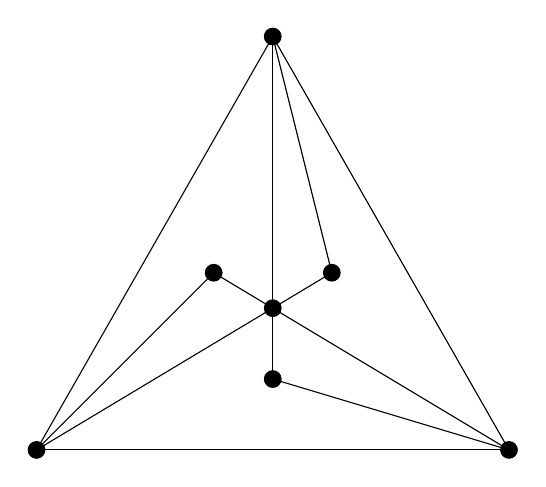
\begin{tikzpicture}[scale=1.5]
\draw (-2,0)--(2,0);

\draw(0,0.6)--(0,3.5);
\filldraw[black](0,1.2) circle(2pt);
\filldraw[black](0,3.5) circle(2pt);
\filldraw[black](-2,0) circle(2pt);
\filldraw[black](2,0) circle(2pt);
\filldraw[black](0.5,1.5) circle(2pt);
\filldraw[black](-0.5,1.5) circle(2pt);
\draw(-2,0)--(0,3.5);
\draw(2,0)--(0,3.5);
\draw(-2,0)--(0.5,1.5);
\draw(2,0)--(-0.5,1.5);
\filldraw[black](0,0.6)circle(2pt);
\draw(0,3.5)--(0.5,1.5);
\draw(-2,0)--(-0.5,1.5);
\draw(0,0.6)--(2,0);



\end{tikzpicture}
\end{center}
\caption{Chv{\'a}tal's example}\label{orispl}
\end{figure}
\newpage




Now, let us look at the series of split graphs $\{G_n\}$. In each $G_n$, the independent set is denoted by $I=\{i_1,i_2,\ldots,l_{2i+1}\}$. The vertices of the clique are $C_1\cup C_2$, where $C_1=\{c^1_1,c^1_2,\ldots,c^1_{2n+1}\}$, and $C_2=\{c^2_1,\ldots,c^2_n\}$. The set of edges is $E(G_n)=\{i_rc^1_r|1\le r\le 2n+1\}\cup\{i_rc^2_s|1\le r\le 2n+1,1\le s\le n\}\cup\{c^i_jc^k_l|c^i_j\neq c^k_l\}$.

Obviously, $G_1$ is exactly Chv{\'a}tal's example. It is not difficult to see that $\{G_n\}$ have no 2-factors. Otherwise, if $G_n$ has one, then there are $4n+2$ edges between $I$ and $C_1\cup C_2$. And there are only $2n+1$ edges between $I$ and $C_1$. This forces the 2-factor to have  $2n+1$ edges between $I$ and $C_2$. Thus there must be some vertices in $C_2$ have at least three edges in the 2-factor. Contradiction.

And it is also easy to check that $$t(G_n)=\min\frac{|S|}{\Omega(G_n-S)}=\min_{1\le r\le 2n}\frac{n+r}{1+r}=\frac{3n}{2n+1},$$where $S$ is any cut-set.
\qed



\subsection{Spider graphs}

Now, let's look at a superclass of the split graphs, i.e. the class of spider graphs. Any reader interested in the topic of spider graphs is recommended to consult \cite{kaiser2007tough} for more details.
\begin{definition}
A graph $G$ is called the intersection graph of subgraphs $H_1,\ldots,H_n$ of a graph $H$ is the vertices of $G$ one-to-one correspond to the subgraphs $H_1,\ldots,H_n$ and two vertices of $G$ is adjacent if and only if the corresponding subgraphs have a common vertex.
\end{definition}
Obviously, we have:
\begin{proposition}
Every graph is an intersection graph of (connected) subgraphs of a graph. 
\end{proposition}
 Now, let look at the definition of {\em spiders} and {\em spider graphs}.
\begin{definition}
A graph is a spider if it is a subdivision of a star. 
\end{definition}
The vertex of a spider of degree greater than two (if any) is called the {\em central vertex} and the paths from its leaves to the central vertex are {\em legs}.
\begin{definition}
A graph $G$ is a spider graph if it is an intersection graph of subtrees of a spider.
\end{definition}

It is easy to prove that:
\begin{proposition}
A split graph is an intersection graph of subtrees of a star (a graph $K_{1,n}$).
\end{proposition}
That means:
\begin{proposition}\label{ss} 
All split graphs are spider graphs.
\end{proposition}

Besides split graphs, there is another subclass of spider graphs, {\em interval graphs}, which are interested by many researchers.
\begin{definition}
A graph is an interval graph if and only if it is an interesction graph of subpaths of a path.
\end{definition}

For interval graphs, there is a remarkable result on the existence of Hamilton cycles, see \cite{keil1985finding}.

\begin{theorem}[Keil 1985]\label{thmintg1th85}
An interval graph $G$ is Hamiltonian if and only if $G$ is 1-tough.
\end{theorem}

Now, let's look at the Hamiltonicity of spider graphs.
\begin{theorem}[Kaiser, Kral and Stacho 2007]\label{spider}
Every $3/2$-tough spider graph $G$ is Hamiltonian.
\end{theorem}
By Proposition \ref{ss}, Theorem \ref{spider} is a generalization of Theorem \ref{split}. By Theorem \ref{spn}, we know that Theorem \ref{spider} cannot be improved.














\subsection{Chordal graphs}\label{secchoginht}



Now, let's look at a generalization of the class spider graphs, chordal graphs.

To understand this relation,we first note the following proposition.
\begin{proposition}
A graph is chordal if and only if it is an intersection graph of subtrees of a tree.
\end{proposition}

That shows:
\begin{proposition}
All spider graphs are chordal.
\end{proposition}



For chordal graphs, there are several remarkable results in the references above.

\begin{theorem}[Chen, Jacobson, Kezdy and Lehel 1997]\label{chord18}
Every 18-tough chordal graph has a Hamilton cycle.
\end{theorem}



On the other hand, there is a result on this topic in the negative direction.
\begin{theorem}[Bauer, Broersma and Veldman 2000]\label{count74ep}
For every $\epsilon>0$, there exists a $(7/4-\epsilon)$-tough chordal non-traceable graph.
\end{theorem}

Since being traceable is a necessary condition of being Hamiltonian, then there exists a $(7/4-\epsilon)$-tough chordal graph who is not Hamiltonian, for any $\epsilon>0$.


\subsubsection{The outline of proof of Theorem \ref{count74ep} (Bauer, Harant and Tkac 1999)}


First, recall the proof of Theorem \ref{exa2000nh}. Whenever we get a graph $H$ which contains no Hamilton path connecting its two vertices $u,v\in H$, we can construct a larger graph $G(H,u,v,l,m)$ which is non-traceable. 

Here, in this situation, we use the following graph (see Figure \ref{t29pic}) as the $H$ in above discussion.

\begin{figure}[h]
\begin{center}
\caption{The graph $H$ for the proof of Theorem \ref{count74ep}}\label{t29pic}
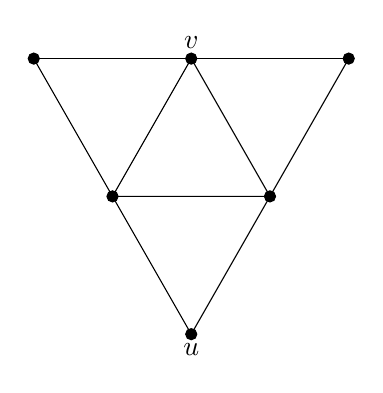
\begin{tikzpicture}

\draw(0,0)--(2,3.5);
\draw(-2,3.5)--(2,3.5);
\draw(0,0)--(-2,3.5);
\filldraw[black](0,0)node[below]{$u$} circle(2pt);
\filldraw[black](0,3.5)node[above]{$v$} circle(2pt);
\filldraw[black](2,3.5) circle(2pt);
\filldraw[black](-2,3.5) circle(2pt);
\filldraw[black](-1,1.75) circle(2pt);
\filldraw[black](1,1.75) circle(2pt);
\draw(-1,1.75)--(1,1.75)--(0,3.5)--(-1,1.75);

\end{tikzpicture}
\end{center}
\end{figure}
\newpage
Similar to the proof of Theorem \ref{exa2000nh}, we can prove that when $m\ge2l+3$ and $l\ge2$, $G(H,u,v,l,m)$ is chordal and has toughness $\frac{7l+9}{4l+7}$. Then we finish the proof.
\qed

Chearly, there is a huge gap between Theorem \ref{chord18} and Theorem \ref{count74ep}. Therefore, much work is to be done on this topic.

However, for planar chordal graphs, there is a nice result in \cite{bohme1999more}.
\begin{theorem}[Bohme, Harant and Tkac 1999]\label{plch}
Every chordal planar graph with toughness greater than 1 is Hamiltonian.
\end{theorem}




\subsection{Planar graphs}

As we have seen in the last section, Hamilton cycles exist in more than 18-tough chordal graphs and more than 1-tough planar chordal graphs. So, being planar seems to be helpful in finding Hamilton cycles. In this section, let us look closely at planar graphs.

First, let us recall Theorem \ref{thm4cpgih1}, which asserts that every 4-connected planar graph is Hamiltonian. Now suppose that a graph $G$ has toughness $t(G)>3/2$, by Proposition \ref{prokg2t}, $\kappa(G)>3$. Because $\kappa(G)$ is always an integer, we get $\kappa(G)\ge4$. Thus, we have:
\begin{theorem}
If a planar graph $G$ has toughness $t(G)>3/2$, then $G$ is Hamiltonian.
\end{theorem}

On the other hand, in 1999, Owens \cite{owens1999nonhamiltonian} constructed a series of examples to show that for any $\delta>0$, there exists a planar graph $G$, with toughness $t(G)>3/2-\delta$, and $G$ is not Hamiltonian.

\begin{theorem}[Owens 1999]\label{cethmow32tnh}
For any integer $k\ge1$, there is a non-hamilton planar graph $G$ with toughness $t(G)=\frac{18k+8}{12k+6}$.
\end{theorem}



\section{Algorithms and their complexity}
In this section, we provide a concise introduction on the complexity of finding Hamilton cycle in graphs. We recommend the readers to consult \cite{cormen2001introduction} for an excellent textbook on algorithms and complexity.


\subsection{P, NP and NP-complete}
Here we informally describe three classes of problems: P, NP and NPC, and we suggest readers to find a more detailed and formal discussion in \cite{cormen2001introduction}.

In most of the time, researchers are interested in the algorithms who are {\em polynomial-time algorithms}: on inputs of size $n$, their worst-case running time is $O(n^k)$ for some constant $k$. However, we know that there are some problems who cannot be solved in polynomial time, for example,  Turing's ``Halting Problem''. We know that it cannot be solved on any computer, regardless how much time we use.

The class P consists of these problems which are solvable in polynomial time. The class NP consists of these problems who are ``verifiable'' in polynomial time. More specifically, if we have a ``certificate'' of a solution, then we could verify that certificate is correct in time polynomial to the size of the input of the problem.
\begin{proposition}\label{hynppo1}
Determining whether a graph has a Hamilton cycle is in the class NP.
\end{proposition}

Undoubtedly, any problem is the class P is also in NP, because if a problem is in P, then it can be solved in polynomial time without any certificate, i.e. $P\subset NP$. It is an open question whether P is a proper subset of NP.

A problem is in the class NP-complete (denoted by NPC for short), if it is in NP and as ``hard'' as any problem in NP. That means if any NP-complete problem can be solved in polynomial time, then every problem in NP has a polynomial time algorithm.

Many interesting problems are {\em optimization problems}, in which each legal solution has a value, and we want to find a feasible solution with the best value. However, NP-completeness applies not to optimization problems, but to {\em decisivion problems}, where the answer is ``yes'' or ``no''.

Technically, we prove a decision problem to be NP-complete if:
\begin{enumerate}
\item it is NP, and
\item every problem in NPC is reducible to it in polynomial time.
\end{enumerate}
As we have seen, in Proposition \ref{hynppo1}, determining whether a graph is Hamiltonian is an NP problem. In fact it is also a NP-complete problem.



\subsection{The complexity of finding Hamilton cycles in some kinds of graphs}

Now, let us look at several examples on the complexity of finding Hamilton cycles in some kinds of graphs.

Recall in Theorem \ref{thmintg1th85}, that an interval graph $G$ is Hamiltonian if and only if it is 1-tough. What is more, Keil also proved that once a Hamilton cycle exists in an interval graph, it can be found in polynomial time.
\begin{proposition}[Keil 1985] 
If an interval graph $G$ contains a Hamilton cycle, then the cycle can be found in time polynomial to $|V(G)|$.
\end{proposition}

For planar graph, it is proved in \cite{gouyou1982hamiltonian} that:
\begin{proposition}[D. Gouyou-Beauchamps 1982]
The problem of determining whether a 4-connected planar graph $G$ is Hamiltonian can be solved in time depending on $|E(G)|^3$.
\end{proposition}


However, when the connectivity becomes lower, the complexity will be higher, for planar graphs. In fact, the following result is found very early in \cite{garey1976planar}.
\begin{proposition}[Garey, Johnson and Tarjan 1976]
It is an NP-complete problem to determine whether a 3-connected cubic planar graph is Hamiltonian.
\end{proposition}

There are also many other examples, in which finding Hamilton cycles is an NP-complete problem. In \cite{krishnamoorthy1975np}, it is proved that:
\begin{proposition}[Krishnamoorthy 1975]\label{popfhcbnpc75}
Finding Hamilton cycles in bipartites is an NP-complete problem.
\end{proposition}

What is more, even assuming the bipartites to be planar, the complexity remains NP-complete \cite{nash1969hamiltonian}.
\begin{proposition}[Nash-Willians 1969]
Finding Hamilton cycles in planar bipartites is an NP-complete problem.
\end{proposition}

Recall Theorem \ref{spn} and Theorem \ref{split} in Section \ref{sec241spg}, we are quite familiar with the Hamiltonicity of split graphs under toughness conditions. However, to determine whether a split graph is Hamiltonian without toughness conditions is a hard problem. The following statement is in fact an exercise in \cite{golumbicalgorithmic}.

\begin{proposition}
To determine whether a split graph is Hamiltonian is an NP-complete problem.
\end{proposition}
\begin{proof}
Obviously, this problem is in NP. So, we only need to find an NPC problem who can be reduced to this problem.

Here we use the fact, Proposition \ref{popfhcbnpc75}, that determining whether a bipartite is Hamiltonian is an NP-complete problem.

Now, we assume there is a polynomial algorithm $\mathcal{A}$, which can determine whether a split graph $H$ is Hamiltonian.
Then for any bipartite $G$, with two parts $M$ and $N$, if $|M|\neq|N|$, then $G$ is certianly not Hamiltonian. 
If $|M|=|N|$, then we add all possible edges between vertices in $N$ to get a clique $\bar{N}$. Then we get a split graph $\bar{G}$, with an independent set $M$ and a clique $\bar{N}$.

Clearly, if $\bar{G}$ is not Hamiltonian, then $G$ is not Hamiltonian either. If the algorithm $\mathcal{A}$ can provide us a Hamilton cycle $\bar{C}$ in $\bar{G}$, then, obviously,  $\bar{C}$ does not use any edge with both endpoints in $\bar{N}$. Therefore $\bar{C}$ induced a Hamilton cycle $C$ in $G$. Then we finish the proof.
\end{proof}







\chapter{Edge-dominating cycles and Hamiltonicity}\label{ch3edcah}
\section{Edge-dominating cycles and long cycles}

Recall that we use $c(G)$ to denote the circumference, i.e. a length of the longest circle, in $G$. A cycle in a graph is a closed walk with each vertex each edge distince. A subset $S\subset V(G)$ is said to be {\em dominating} in $G$, if $S^{\perp}=S\cup N(S)=V(G)$.

\begin{definition}
A cycle $C$ in a graph $G$ is called edge-dominating, if the induced subgraph $G-C$ is a coclique.
\end{definition}
Clearly, in any connected graph $G$, an edge-dominating cycle is a dominating cycle as well.

\subsection{Long cycles in graphs}

Obviously, assume $|V(G)|=n$, then $G$ is Hamiltonian if and only if $c(G)=n$. Additionally, a Hamilton cycle is trivially a dominating cycle and an edge-dominating cycle.

The first result in this topic should be the following one by Dirac:



\begin{theorem}[Dirac]
Let $G$ be a 2-connected graph on $n$ vertices, then $c(G)\ge\min\{n,2\delta\}$.
\end{theorem}

In a graph $G$, for any $k\le\alpha(G)$, we denote $\sigma_k(G)$ to be the minimum degree sum taken over all independent sets of $k$ vertices of $G$.
Then the theorem above can be generalized \cite{linial1976lower} into:
\begin{theorem}[Linial 1976]
Let $G$ be a 2-connected graph on $n$ vertices. Then $c(G)\ge\min\{n,\sigma_2\}$.
\end{theorem}


In \cite{bauer1987long} Bauer and Schmeichel found a similar result:
\begin{theorem}[Bauer, Schmeichel 1987]\label{bauschd2}
Let $G$ be a 1-tough graph on $n\ge3$ vertices. Then $c(G)\ge \min\{n,\sigma_2+2\}$.
\end{theorem}








\subsection{Edge-dominating cycles in graphs}

The concept of edge-dominating cycles is very important in the research of Hamiltonicity. This concept was first introduced by Nash-Williams in around 1970. In \cite{nash1971edge}, Nash-Williams proved:
\begin{theorem}[Nash-Williams 1971]\label{nashd}
Let $G$ be a 2-connected graph on $n$ vertices with $\delta\ge(n+2)/3$. Then every longest cycle in $G$ is an edge-dominating cycle.
\end{theorem}


In \cite{bondy1980longest}, Bondy generalized the theorem above to the following form.

\begin{theorem}[Bondy 1980]\label{bong}
Let $G$ be a 2-connected graph on $n$ vertices with $\sigma_3\ge n+2$. Then every longest cycle in $G$ is an edge-dominating cycle.
\end{theorem}

Under the same assumption, Bauer, Morgana, Schmeichel and Veldman proved another result \cite{bauer1990long}.
\begin{theorem}[Bauer, Morgana, Schmeichel and Veldman 1990]\label{bmsv3}
Let $G$ be a 2-connected graph on $n$ vertices with $\sigma_3\ge n+2$. Then $c(G)\ge\min\{n,n+\sigma_3/3-\alpha\}$.
\end{theorem}

Changing 2-connected condition in Theorem \ref{nashd} into 1-tough condition, Bigalke and  Jung proved that:

\begin{theorem}[Bigalke, Jung 1979]
Let $G$ be a 1-tough graph on $n$ vertices with $\delta\ge n/3$. Then every longest cycle in $G$ is an edge-dominating cycle.
\end{theorem}


Similar to Theorem \ref{bong}, the above theorem is generalized into the following form \cite{bauer1990long}:
\begin{theorem}[Bauer, Morgana, Schmeichel and Veldman 1990]\label{bmsvtou}
Let $G$ be a 1-tough graph on $n$ vertices with $\sigma_3\ge n$. Then every longest cycle in $G$ is an edge-dominating cycle.

\end{theorem}

In \cite{bauer1995long}, this theorem is generalized into $t$-tough version:
\begin{theorem}[Bauer, Broersma, Heuvel and Veldman 1995]\label{bbhvtt}
Let $G$ be a $t$-tough graph ($t\ge1$) on $n\ge3$ vertices with $\delta>n/(t+2)$. Then $G$ contains an edge-dominating cycle.
\end{theorem}


In \cite{veldman1983existence}, Veldman established a remarkable theorem on the existence of edge-dominating cycles under some requirements on remote edges. For $e\in E(G)$, let $d(e)$ stand for the number of edges sharing vertex with $e$.
We say two subgraphs (or edges) $H_1$ and $H_2$ in $G$ are {\em remote}, if:
\begin{enumerate}
\item $H_1$ and $H_2$ are vertex-disjoint, and
\item there is no edge incident to one vertex in $H_1$ and one vertex in $H_2$.
\end{enumerate}
\begin{theorem}[Veldman 1983]\label{veldmanfound1}
For any $k$-connected graph $(k\ge2)$, if every $k+1$ pairwise remote edges $e_0,\ldots,e_k$ have $$\sum^k_{i=0}d(e_i)>\frac{k(|V(G)|-k)}{2},$$
then $G$ admits an edge-dominating cycle.
\end{theorem}

\begin{proof}
Here, we only describe the outline of the proof, we strongly recommend the readers who are interested in this result to consult \cite{veldman1983existence} for the detailed proof.

The proof uses contraposition. Assuming $G$ is a $k$-connected graph with no edge-dominating cycle, we need to show that there is a set of $k+1$ vertex-disjoint edges with degree-sum at least $\frac{k(|V(G)|-k)}{2}$.

Suppose $C$ is a longest cycle in $G$. Then through Menger's Theorem (Theorem \ref{mengert27}), we can deduce that $C$ has length at least $k+1$.

Now, suppose $u_{01}u_{02}$ is an edge of $G-V(C)$ and $\mathcal{P}=\{P_1,\ldots,P_m\}$ is a maximum set of inner-vertex-disjoint  paths with one endpoint $u_{01}$, another endpoint (pairwise different) on $C$. Additionally, these paths have no inner vertex on $C$.


With the help of these concepts, we can find a set of edges $F=\{e_i|i=0,1,\ldots,m\}\subset E(G)$ satisfying:
\begin{enumerate}
\item $d(e_0)+d(e_i)+d(e_j)\le|V(G)|-2$,
\item $d(e_i)+d(e_j)\le|V(G)|-k-2$,
\item $d(e_0)\ge k$.
\end{enumerate}

Finally, we get $$\sum^k_{i=0}\le\frac{k(|V(G)|-k)}{2}).$$

Then we have finished the proof.

\end{proof}

From this result, we can easily deduce that

\begin{corollary}\label{cor2k2edgd}
Suppose $G$ is a $2K_2$-free graph (a graph without any pair of remote edges), and if $G$ is not a tree, then $G$ admits an edge-dominating cycle.
\end{corollary}

\begin{corollary}\label{co32c3kfed}
Every 2-connected $3K_2$-free graph $G$ admits an edge-dominating cycle.
\end{corollary}



\subsection{Edge-dominating 2-factors in graphs}

As we have seen, a 2-factor is a natural generalization of a Hamilton cycle. So, in this section, let us look at a recent result by Fujita, Saito and Yamashita \cite{fujita2007edge}, which talks about the existence of edge-dominating 2-factors.

An {\em edge-dominating 2-factor} $\mathcal{F}$ in a graph $G$ is a (not necessarily spanning) subgraph who is the union of some disjoint cycles, and such that the induced subgraph $G-\mathcal{F}$ contains no edge.

\begin{theorem}[Fujita, Saito and Yamashita 2007]\label{thmed2f1}
For any positive integer $k$, assume 2-connected graph $G$ has $n\ge44$ vertices and contains at least $k$ disjoint cycles as subgraphs. And if the minimum degree $\delta(G)\ge\frac{n+2}{3}$, then for every maximum subgraph $\mathcal{F}$ of $k$ disjoint cycles, we have $\mathcal{F}$ is edge-dominating. Here we say $\mathcal{F}$ is maximum if there is not another subgraph $\mathcal{F}'$ of $G$ consisting of $k$ disjoint cycles with $|V(\mathcal{F}')|>|V(\mathcal{F})|$.
\end{theorem}

The proof of this theorem is highly tricky, so we do not include it here, and we recommend the readers to consult \cite{fujita2007edge} for the detailed proof.









\subsection{Edge-dominating cycles and line graphs}
Now, let us look at another application of edge-dominating cycles. Edge-dominating cycles are very important in the research of Hamiltonicity in line graphs.

\begin{definition}
For a graph $H$, the line graph of $H$, denoted as $L(H)$, is the graph on vertex set $E(H)$ in which two vertices in $L(H)$ are adjacent if and only if their corresponding edges in $H$ share an end vertex (with a straighforward extension in case of multiple edges).
A graph $G$ is a line graph if it is isomorphic to $L(H)$ for some graph $H$.
\end{definition}


The following theorem \cite{harary1965eulerian}, explains the importance of edge-dominating cycles in the research of line graphs.

\begin{theorem}[Harary, Nash-Williams 1965]\label{edmtraitohalig}
The line graph $L(G)$ of $G$ is Hamiltonian if and only if either $G$ admits an edge-dominating trail or $G$ is isomorphic to $K_{1,s}$ for some $s\ge3$.
\end{theorem}


\begin{proof}

For one direction, assuming $G$ is isomorphic to $K_{1,s}$ for some $s\ge3$, then obviously the line graph $L(G)$ is exactly $K_s$, the complete graph. What is more, if $G$ contains an edge-dominating trail $T$, then we can go along this trail and pick up the edges outside this trail one by one. Obviously, the line graph $L(G)$ is Hamiltonian.

For another direction, once we get a Hamilton cycle in $L(G)$, and assume $G$ is not isomorphic to $K_{1,s}$, then the Hamilton cycle in $L(G)$ easily induced a edge-dominating cycle in $G$.

\end{proof}
Obviously, an edge-dominating cycle is strictly stronger than an edge-dominating trail. So, we have:
\begin{corollary}\label{edmctohlg}
If $G$ admits an edge-dominating cycle, then $L(G)$ is Hamiltonian.
\end{corollary}

If a graph $G$ admits an edge-dominating path $P$ with endpoints $v_1$ and $v_2$, then the graph $G+v_1v_2$ contains an edge-dominating cycle, $P+v_1v_2$. Thus, $L(G+v_1v_2)$ has a Hamilton cycle. Because $L(G)$ is obtained from $L(G+v_1v_2)$ by deleting the vertex corresponding to the edge $v_1v_2$, then $L(G)$ contains a Hamilton path.
\begin{corollary}
If $G$ admits an edge-dominating path, then $L(G)$ contians a Hamilton path.
\end{corollary}



\section{Line graphs and claw-free graphs}\label{seclandclfg}


\subsection{Introduction}
In this part, we talk about some results, old or recent, on the Hamiltonicity of line graphs and claw-free graphs.
\begin{definition}
A graph $G$ is claw-free if $G$ does not contain a copy of the claw $K_{1,3}$ as an induced subgraph.
\end{definition}
In this topic, people are most interested in the Hamiltonicity of these graphs under some connectivity conditions rather than toughness conditions.
However, by Proposition \ref{prokg2t} there is a close relation between connectivity and toughness.



Most of the recent researches on this topic are concentrated on the following two famous conjectures:
\begin{conjecture}[Matthews and Summer 1984]\label{4clf}
Every 4-connected claw-free graph is Hamiltonian
\end{conjecture}


\begin{conjecture}[Thomassen 1986]\label{4lineh}
Every 4-connected line graph is Hamiltonian.
\end{conjecture}

Any reader, who is interested in this topic, is recommended to consult \cite{broersma2012many} for further information. 






\subsection{The equivalence between Conjecture \ref{4clf} and Conjecture \ref{4lineh}}
First, a corollary of the main theorem of \cite{beineke1970characterizations} tells us:

\begin{theorem}[Beineke 1970]\label{2to3}
Every line graph $G$ is a claw-free graph.
\end{theorem}

In another direction, Ryj{\'a}{\v{c}}ek, Zden{\v{e}}k introduced a closure concept for claw-free graphs in 1997, see \cite{ryjavcek1997closure}. Similar to the Bondy-Chv{\'a}tal closure, its main idea is adding edges without changing the Hamiltonicity.

For any vertex $v\in G$, if the induced subgraph $G|_{N(v)}$ on the neighborhood $N(v)$ of $v$ is connected and not a complete graph, then add all edges to make $G|_{N(v)}$ into a complete graph. Repeat this procedure in the new graph, until it is impossible to add any more edges. The result after this process is called the {\em closure} of $G$, denoted as $cl(G)$.

For the closure of a graph, we have:
\begin{theorem}[Ryj{\'a}{\v{c}}ek, Zden{\v{e}}k 1997]\label{3to2}
Let $G$ be a claw-free graph, then
\begin{enumerate}
\item the closure $cl(G)$ is uniquely determined,
\item $cl(G)$ is the line graph of a triangle-free graph,
\item $cl(G)$ is Hamiltonian if and only if $G$ is Hamiltonian.
\end{enumerate}
\end{theorem}

The following lemma is useful in the proof of Theorem \ref{3to2}, and also of independent interest.

\begin{lemma}[Ryj{\'a}{\v{c}}ek, Zden{\v{e}}k 1997]\label{3to2lm1}
Let $G$ be a graph such that, for every $x\in V(G)$, $G[N(x)]$ is either a clique or a disjoint union of two cliques. Then there is a triangle-free graph $H$ such that $G=L(H)$.
\end{lemma}

From Theorem \ref{2to3} and Theorem \ref{3to2}, we can deduce that Conjecture \ref{4clf} and Conjecture \ref{4lineh} are indeed equivalent.
Now, let us look at some other conjectures, which may seem stronger or weaker, but are equivalent to these two conjectures above.

\subsection{Some other equivalent conjectures}
\begin{definition}
An {\em edge-dominating closed trail} $T$ in $G$ is a closed trail (also called circuit sometimes) $T$ such that every edge in $G$ has at least one end vertex on $T$.
\end{definition}

The following theorem, in \cite{harary1965eulerian}, is both famous and important.

\begin{theorem}[Harary, Williams 1965]\label{dctl}
Let $G$ be a graph with at least three edges. Then $L(G)$ is Hamiltonian if and only if $G$ contains an edge-dominating closed trail.
\end{theorem}


In \cite{fleischner1988note}, Fleischner and Jackson proved the following conjecture is equivalent to Conjecture \ref{4clf} and Conjecture \ref{4lineh}.


\begin{conjecture}[Fleischner, Jackson 1989]\label{flejac}
Every cyclically 4-edge-connected cubic graph has a dominating cycle.
\end{conjecture}


In \cite{kochol2000equivalence}, Kochol proved that these conjectures above are equivalent to the following one.
\begin{conjecture}[Kochol 2000]\label{kochole}
Every cyclically 4-edge-connected cubic graph that is not 3-edge-colorable has a dominating cycle.
\end{conjecture}

In \cite{broersma2008contractible}, it is proved that the following conjecture, although appearing independently at different places, is also equivalent to the conjectures above.

\begin{conjecture}
Every snark has a dominating cycle
\end{conjecture}
Here a {\em snark} is defined as a cyclically 4-edge-connected cubic graph of girth at least 5 that is not 3-edge-colarable.


Also in \cite{broersma2008contractible}, the authors posed another conjecture that is equivalent to the others.

\begin{conjecture}[Broersma, Fijav{\v{z}}, Kaiser, Ku{\v{z}}el, Ryj{\'{a}}{\v{c}}ek and Vr{\'{a}}na 2008]\label{bfkkrv}
Every cyclically 4-edge-connected cubic graph contains a weakly contractible subgraph $F$ with $\delta(F)=2$.
\end{conjecture}


In \cite{fouquet1990some}, Fouquet and Thuillier posed another equivalent, although seemingly stronger, conjecture as follows.

\begin{conjecture}[Fouquet, Thuillier 1990]\label{fouthui}
In a cyclically 4-edge-connected cubic graph any two disjoint edges are on a dominating cycle.

\end{conjecture}


In 2004, Ku{\v{z}}el and Xiong find another equivalent conjecture.

\begin{conjecture}[Ku{\v{z}}el and Xiong 2004]\label{kuxio}
Every 4-connected line graph of a multigraph is Hamilton-connected.
\end{conjecture}

In \cite{ryjavcek2011line}, Ryj{\'{a}}{\v{c}}ek and Vr{\'{a}}na pointed out the following conjecture is equivalent to the conjectures above.
\begin{conjecture}[Ryj{\'{a}}{\v{c}}ek and Vr{\'{a}}na 2010]\label{ryjvr}
Every 4-connected claw-free graph is Hamilton-connected.
\end{conjecture}







\section{$D_{\lambda}$-cycles}

In this section, we discuss the $D_{\lambda}$-cycle, which is a generalization of the concept edge-dominating cycle, introduced by Veldman in 1983 \cite{veldman1983existence2}.

\begin{definition}
A cycle $C$ in a graph $G$ is said to be a $D_{\lambda}$-cycle, if each component of the induced subgraph $G-V(C)$ contains less than $\lambda$ vertices.
\end{definition}

Obviously, we have the following proposition equivalent to the definition.
\begin{proposition}
A cycle $C$ in $G$ is a $D_{\lambda}$-cycle if and only if each connected subgraph with $\lambda$ vertices has at least one vertex on $C$.
\end{proposition}

Clearly, a $D_1$-cycle is a Hamilton cycle and a $D_2$ cycle is an edge-dominating cycle.
In \cite{veldman1983existence2}, Veldman gave the following results on $D_{\lambda}$-cycles.
\begin{proposition}\label{thm1inveldlamc83}
Suppose a graph $G$ contains a $D_{\lambda}$-cycle, then for any non-empty proper subset $S\subset V(G)$, we have $\Omega_{\lambda}(G-S)\le|S|$, where $\Omega_{\lambda}(G-S)$ stands for the number of components in $G-S$ with at least $\lambda$ vertices.
\end{proposition}

Let $\alpha_{\lambda}(G)$ stand the maximum number of pairwise remote connected subgraph with $\lambda$ vertices of $G$.

\begin{theorem}[Veldman 1983]\label{thm2inveldlamc83}
Suppose $k$ and $\lambda$ are two positive integers and $G$ is a $k$-connected non-tree graph. If:
\begin{enumerate}
\item $k\ge2$, or
\item $k=1$ and $\lambda\le2$,
\end{enumerate}
and if $\alpha_{\lambda}\le k$, then $G$ has a $D_{\lambda}$-cycle.
\end{theorem}

\begin{theorem}[Veldman 1983]\label{thm3inveldlamc83}
Suppose $k$ and $\lambda$ are two positive integers and $G$ is a $k$-connected non-tree graph. If:
\begin{enumerate}
\item $k\ge2$, or
\item $k=1$ and $\lambda\le2$,
\end{enumerate}
and if for any $k+1$ pairwise remote connected subgraphs of $G$, say $H_0,H_1,\ldots,H_k$, with $\lambda$ vertices, satisfy $$\sum^k_{i=0}d(H_i)>\frac{(k+1)(|V(G)|+k-\lambda-k\lambda)}{2},$$
then $G$ admits a $D_{\lambda}$-cycle.

\end{theorem}
In a graph $G$, let $\delta_{\lambda}(G)$ stand for the mimimum degree of connected subgraphs of $G$ with exactly $\lambda$ vertices.
\begin{theorem}[Veldman 1983]\label{thm4inveldlamc83}
Suppose $k$ and $\lambda$ are two positive integers and $G$ is a $k$-connected non-tree graph. If:
\begin{enumerate}
\item $k\ge2$, or
\item $k=1$ and $\lambda\le2$,
\end{enumerate}
and if $$\delta_{\lambda}>\left\{\begin{array}{cc}\frac{|V(G)|-(k+1)\lambda+k^2}{k+1}&\text{if }\lambda\ge k,\\ \frac{|V(G)|-\lambda}{\lambda+1}&\text{if }\lambda\le k,\end{array}\right.$$
then $G$ contains a $D_{\lambda}$ cycle.
\end{theorem}

\begin{theorem}[Veldman 1983]\label{thm5inveldlamc83}
Suppose a graph $G$ is 2-connected and the degree-sum of any three pairwise remote connected subgraphs with $\lambda\ge2$ vertices is at least $|V(G)|-3\lambda+5$. Then $G$ contains a $D_{\lambda}$-cycle.

\end{theorem}










\chapter{$k$-walks in a Graph}\label{ch4kw}
In this chapter, we investigate another generalization of Hamilton cycles, the $k$-walks. 
\begin{definition}\label{defkwalk}
A $k$-walk in a graph $G$ is a spanning closed walk which visiting each vertex in $G$ at most $k$ times.
\end{definition}

Clearly, for any graph on at least 3 vertices, a 1-walk is a Hamilton cycle.





\section{$k$-trees, $k$-walks and Hamilton cycles}\label{sectionktwh}


In a connected graph $G$, a {\em $k$-tree} is a spanning tree with maximum degree at most $k$. Obviously, when $k=2$, this tree is a Hamilton path.

Around 25 years ago, two excellent papers, \cite{win1989connection} by Sien Win and \cite{jackson1990k} by Jackson and Wormald, laid the fundation of the research on this topic. So, most results in this section are selected from this two papers. And interested readers are recommended to consult them.

In this section, we discuss the relation between the toughness and the existence of $k$-trees and $k$-walks. The following two theorems are the main topic in this section.
\begin{theorem}[Sien Win 1989]\label{tktree}
For any integer $k\ge3$, if the toughness of graph $G$, $t(G)\ge\frac{1}{k-2}$, then $G$ admits a $k$-tree.
\end{theorem}

\begin{theorem}[Jackson, Wormald 1990]\label{ktreetokwalk}
For any connected graph $G$,
\begin{enumerate}

\item if $G$ admits a $k$-tree, then $G$ contains a $k$-walk,

\item if $G$ admits a $k$-walk, then $G$ has a $(k+1)$-tree,

\item if $G$ admits a $k$-walk, then $G$ is $\frac{1}{k}$-tough.
\end{enumerate}
\end{theorem}


In fact, in \cite{win1989connection}, Sien Win proved a slight stronger version of Theorem \ref{tktree}.
\begin{theorem}[Sien Win 1989]\label{tktreeslistr2}
If integer $k\ge2$, $G$ is a connected graph and for any subset $S\subset V(G)$, the number of components in $G-S$, $\Omega (G-S)\le(k-2)|S|+2$, then $G$ has a $k$-tree.
\end{theorem}

Then we have the following obvious corollary.
\begin{corollary}\label{cor24injw90}
In a connected graph $G$, when integer $k\ge2$, if for any subset $S\subset V(G)$, we have $\Omega(G-S)\le(k-2)|S|+2$, then $G$ admits a $k$-walk.
\end{corollary}









\section{$k$-walks for some special graphs}

\subsection{$k$-walks under some claw-free type conditions}

Usually, when we expect a graph to have a $k$-walk, we may require some toughness-condition to hold, as we shall see in the following sections. However, we list some results on $k$-walks without such a requirement.

As we have seen in the chapter before, the claw-free condition attracts much attention in the research on Hamiltonicity. What is more, claw-free graphs and their generalization, $K_{1,n}$-free graphs have many advantages in the topic of $k$-walks.

\begin{theorem}[Jackson, Wormald 1990]\label{k1kfkwalk}
Any connected $K_{1,k+1}$-free graph admits a $k$-walk.
\end{theorem}
\begin{proof}
Recall that $\alpha(G)$ stands for the independent number of a graph $G$. Denote the induced subgraph on all the neighbors of a vertex $v\in G$ by $G|_{N(v)}$. The maximum degree of a graph $G$ is denoted by $\Delta (G)$ as usual. Now, suppose $G$ is connected. To prove this theorem, we need to show that there exists a connected spanning subgraph $W$, with all vertex degree even, of $m*G$, such that $d_W(v)$ is at most $2\alpha(G|_{N(v)})$ for any $v\in V(G)$.

First, let $W$ be a $\Delta(G)$-walk (it certainly exists) of $G$ for which $|E(G)|$ is minimised.
If there exists a vertex $v$ such that $d_W(v)=2r>2\alpha(G|_{N(v)})$, we choose an Euler tour, namely $T$. Let $y_1,\ldots,y_r$ stand for the edges incident to $v$ in different branches of $T$ at $v$. We claim that there is a $\Delta(G)$-walk $W'$ of $G$ such that $|E(W')|<|E(W)|$. Note that $W-\{y_1,\ldots,y_r\}$ is a connected graph, since in each branch, there remais an edge. Now, if there are some $y_i$ and $y_j$ (with $i\neq j$) having the same endpoint, then we can delete them from $W$ to get a $W'$ as required. Otherwise, $y_1,\ldots,y_r$ are incident to exactly $r>\alpha(G|_{N(v)})$ different vertices, namely $w_1,\ldots,w_r$ in $N(v)$. So there is some $w_iw_j\in E(G)$ with $i\neq j$. Then we get $W'=W-y_i-y_j+w_iw_j$ as required. This contradicts with the assumption that $|E(W)|$ is minimised.



\end{proof}

Obviously, $K_{1,k}$ has no $(k-1)$-walk, so Theorem \ref{k1kfkwalk} is sharp.

With some better connectivity-condition, the $K_{1,k}$-free condition can be weaken. We say a graph $G$ is {\em locally connected}, if for any $v\in V(G)$, we have the induced subgraph on $N(v)$ is connected.

\begin{theorem}[Jackson, Wormald 1990]\label{k1k2fkw}
For an integer $k\ge1$, every connected, locally connected $K_{1,k+2}$-free graph on at least two vertices admits a $k$-walk.
\end{theorem}

This theorem generalizes a result in \cite{oberly1979every}.
\begin{theorem}[Oberly, Sumner 1979]\label{k13flnh}
Every connected, locally connected claw-free graph on at least three vertices is Hamiltonian.
\end{theorem}

If given stronger global connectivity, there is stronger result.

\begin{theorem}[Jackson, Wormald 1990]\label{globconkw}
For integers $j\ge1$, $k\ge3$, any $j$-connected $K_{1,j(k-2)+1}$-free graph $G$ admits a $k$-walk.
\end{theorem}


\begin{proof}
In a $j$-connected graph $G$, for any proper subset $S\subset V(G)$, each component of $G-S$ is adjacent to at least $j$ vertices in $S$. Because $G$ is a $K_{1,j(k-2)+1}$-free graph, each vertex in $S$ is adjacent to at most $j(k-2)$ components of $G-S$. Therefore $\Omega(G-S)\le(k-2)|S|$. Then by Corollary \ref{cor24injw90}, we get the result we want.



\end{proof}

Moreover, Jackson and Wormald believed this theorem can be improved.

\begin{conjecture}\label{jck1jkfc}
For integers $j\ge1$, $k\ge2$, and $j$-connected $K_{1,jk+1}$-free graph $G$ admits a $k$-walk.
\end{conjecture}

However, in 2004, Jin and Li disproved this conjecture by constructing a counterexample \cite{jin2004conjecture}.
\subsubsection{A counterexample for Conjecture \ref{jck1jkfc} (Jin, Li 2004)}
Jin and Li's counterexample is based on a result by Meredith \cite{meredith1973regular}. Roughly speaking, Meredith proved the following result in \cite{meredith1973regular}.
\begin{theorem}[Meredith 1973]\label{mergenthm1}
For any integer $j\ge3$, there exist $j$-connected and $j$-regular non-hamilton graphs.
\end{theorem}



The counterexamples for Conjecture \ref{jck1jkfc} are constructed as follows. Suppose $G$ is a $j$-connected, $j$-regular, non-hamilton graph for some $j\ge3$. For each $x\in V(G)$, we make $jk-1$ new vertices $x^1,x^2,\ldots,x^{jk-1}$, and for every edge $\alpha\in E(G)$ who is incident to $x$, we make a new vertex $x_{\alpha}$.

Now, denote
$$D(x)=\{x_{\alpha}|\alpha\in E(G)\text{ and is incident to }x\},$$
$$S(x)=\{x^i|i=1,2,\ldots,jk-1\}.$$
Clearly, $|D(x)|=d_G(x)=j$ and $|S(x)|=jk-1$. We construct a new graph $G^*$ as follows:
$$V(G^*)=\cup_{x\in V(G)}(D(x)\cup S(x)),$$
$$E(G^*)=E_1\cup E_2,$$
where
$$E_1=\{x_{\alpha}y_{\alpha}|\alpha=xy\in E(G)\},$$
and
$$E_2=\{uv|u\in D(x),v\in S(x)\text{ for some }x\in V(G)\}.$$
From the construction, we know that $G^*$ is $j$-connected and $K_{1,jk+1}$-free. Now, let us prove that $G^*$ does not contain any $k$-walk.

If $G^*$ contains a $k$-walk, say $W$. Then we shall show for each vertex $x\in V(G)$, there is a sub-walk $w_x=v_1v_2\cdots v_{2jk-1}$ in $W$ such that $S(x)=\{v_{2i}|1\le i\le jk-1\}$ and $D(x)=\cup_{i=1}^{jk}\{v_{2i-1}\}$.

Otherwise, in order to visit all vertices in $S(x)$, the sum of the visiting times of vertices in $D(x)$ is at least $|S(x)|+2=jk+1$. Because $N_G(S(x))=D(x)$ and both $D(x)$ and $S(x)$ are independent set in $G^*$, there is at least one vertex in $D(x)$ which is visited by $W$ at least $k+1$ times. Contradition.

Thus each vertex of $D(x)$ is visited exactly $k$ times, because the sum of visiting times of all vertices in $D(x)$ is $|S(x)|+1=jk$ and $|D(x)|=j$. We can denote $W$ by $x_{\alpha}W_{x_1}W_{x_2}\ldots W_{x_n}y_{\alpha}$, with $n=|V(G)|$, $x=x_1$, $y=x_n$, $\alpha=xy\in E(G)$ and $x_i\neq x_l$ for $i\neq l$. Because $W$ is a $k$-walk, there must be an edge $e_i\in E(G)$ such that $e_i=x_ix_{i+1}$ for any $1\le i\le n-1$. So, we get a Hamilton cycle of $G$. Contradiction.
\qed





































\subsection{$k$-walks under some minimum-degree type conditions}
Recall Theorem \ref{dirac1952th}, which claims that every graph $G$ on at least three vertices with minimum degree at least $\frac{V(G)}{2}$ has a Hamilton cycle. Jackson and Wormald provided a $k$-walk type generalization.

\begin{theorem}[Jackson, Wormald 1990]\label{mindekwa1}
Suppose $G$ is a connected graph, with minimum degree $\delta(G)\ge\frac{|V(G)|-1}{k+1}$, then $G$ admits a $k$-walk.
\end{theorem}

\begin{proof}
Let $G[K_k]$ stand for the composition of $G$ and $K_k$, i.e. changing each vertex in $G$ into a clique $K_k$, and two vertices of $G[K_k]$ in different clique are adjacent if and only if their corresponding vertices in $G$ are adjacent. We observe that $G$ admits a $k$-walk if $G[K_k]$ contains a $D_k$-cycle. Clearly, $G[K_k]$ is $k$-connected, and $|V(G[K_k])|=k|V(G)|$. Note that every subgraph $F$ of $G[K_k]$ with $k$ vertices has more than $\frac{k(|V(G)|-1)}{k+1}$ neighbors in $V(G[K_k])-V(F)$. Then by Theorem \ref{thm4inveldlamc83}, $G[K_k]$ contains a $D_k$-cycle.




\end{proof}


What is more, there is a generalization of the Ore-type result, i.e. Theorem \ref{ore1960hth1}, as well.

\begin{theorem}[Jackson, Wormald 1990]\label{oretjacw1}
For any connected graph $G$, if any set of $k+1$ independent vertices in $G$ have degree sum at least $|V(G)|$, then $G$ admits a $k$-walk.
\end{theorem}


Theorem \ref{oretjacw1} has the following trivial corollary.
\begin{corollary}\label{cooretjacw1}
Every connected graph $G$ admits an $\alpha(G)$-walk.
\end{corollary}


Moreover, There is a generalization on higher connectivity.

\begin{theorem}[Jackson, Wormald 1990]\label{alphkwjc1}
For any $j$-connected graph $G$. Denote $k=\lceil\alpha(G)/j\rceil$, then $G$ admits a $k$-walk.
\end{theorem}


\begin{proof}
Similar to the proof of Theorem \ref{mindekwa1}, we consider $G[K_k]$ again. Obviously, $G[K_k]$ is $kj$-connected. Thus $\kappa(G[K_k])\ge\alpha(G[K_k])$. By Theorem \ref{kageaptohathe}, $G[K_k]$ is Hamiltonian. Obviously, the Hamilton cycle in $G[K_k]$ induces a $k$ walk in $G$.
\end{proof}

Clearly, Theorem \ref{thmce15} can be considered as a corollary of this result.
























\subsection{$k$-walks in bridgeless graphs}

In this section, we look at a concrete example on $k$-walks in graphs. Recall Definition \ref{bilede}, we say a graph $G$ is {\em bridgeless}, if it does not contain any bridge. 

In \cite{kaiser2007note}, Kaiser, Kuz{\v{e}}l, Li and Zhang proved that every bridgeless graph of maximum degree $\Delta$ admits a $\lceil(\Delta+1)/2\rceil$-walk. and the bound is the best possible.
Now, for a walk $W$ in graph $G$, let $p_W(v)$ denote the number of times walk $W$ visits vertex $v\in V(G)$.
\begin{theorem}[Kaiser, Kuz{\v{e}}l, Li and Zhang 2007]\label{kwiblgub1}
Every bridgeless graph $G$ contains a spanning walk $W$ such that for every vertex $x\in V(G)$, $p_W(x)\le\lceil\frac{deg(x)+1}{2}\rceil$.

\end{theorem}

\begin{theorem}[Kaiser, Kuz{\v{e}}l, Li and Zhang 2007]\label{kwiblglb2}
For any $\Delta\ge4$, there is a 2-connected graph $G$ with $\Delta(G)=\Delta$ and no $\frac{\Delta}{2}$-walk.
\end{theorem}

\subsubsection{Some lemmas}
Here we list some lemmas which will be used in the proof of Theorem \ref{kwiblgub1}.
Assume two edges in $G$ $e_1$, $e_2$ are incident with a vertex $v\in V(G)$. Let $v_i$ be the endvertex of $e_i$ distince from $v$. We define the operation of {\em splitting} $e_1$ and $e_2$ off $v$. The resulting graph, denoted by $G(v,e_1,e_2)$ is defined to be $G$ with an added vertex $v^*$ and the edges $e_1$, $e_2$ replaced by $e_1^*$, $e_2^*$, where $e_i^*$ has ends $v^*$ and $v_i$. 

\begin{lemma}\label{lm2inbri}
Let $v$ be a vertex of degree at least in a bridgeless graph $G$. There exist edges $e_1$, $e_2$ incident with $v$ such that the graph $G(v,e_1,e_2)$ is bridgeless. 
\end{lemma}


\begin{lemma}[Kaiser, Kuz{\v{e}}l, Li and Zhang 2007]\label{lm3inbri}
For any vertex $v\in V(G)$, let $e_1$, $e_2$ be two edges incident with $v$, and $H=G(v,e_1,e_2)$. If $W$ is a spanning closed walk in $H$ such that $p_W(v^*)\le2$, then $G$ contains a walk $\tilde{W}$ such that
\begin{enumerate}
\item for all $x\in V(G)-\{v\}$, $p_{\tilde{W}}(x)\le p_W(x)$,
\item $1\le p_{\tilde{W}}\le p_W(v)+1$.
\end{enumerate}
\end{lemma}

Now, let us define a function on edge-set of a graph, called {\em Euler weight}.





\begin{lemma}[Kaiser, Kuz{\v{e}}l, Li and Zhang 2007]\label{lm4inbri}
Let $G$ be a graph and $k\ge1$ be a positive integer. The graph $G$ admits a $k$-walk if and only if it contains an Euler weight $w(e)$ such that for any $v\in V(G)$, $w(\partial v)\le 2k$.
\end{lemma}

\begin{proof}
For the first part, let $W$ stand for a $k$-walk in $G$. Then the function assigning every edge the number of times it is used by $W$ is certainly an Euler weight with $w(\partial v)\le 2k$, for any $v\in V(G)$.

On the other hand, suppose $w$ is such a Euler weight. Let us replace each edge $e$ by $w(e)$ parallel edges (or deleting it if $w(e)=0$) to obtain a connected Euler graph with maximum degree at most $2k$. Then any Euler trail in the new graph determines a $k$-walk in $G$.
\end{proof}



\subsubsection{The proof of Theorem \ref{kwiblgub1}}
The proof uses mathematical induction. First we shall show the result is true when $\Delta(G)\le3$. Then we prove, if $\Delta(G)\ge4$, the result is true for $G$ under the assumption it is true for all bridgeless graphs that are smaller than $G$.

Now, suppose $\Delta(G)\le3$. For $G$ is bridgeless, so the minimum degree $\delta(G)$ is at least 2. Therefore $G$ can be considered as a subdivision of a cubic bridgeless graph $H$. By Theorem \ref{petbrile1fa}, $H$ contains a 1-factor, namely $F$. Denote $w:E(G)\rightarrow\{1,2\}$ to be a function whose value is 2 if the edge of $H$ corresponding to $e$ is in $F$, and 1 otherwise. We can see that $w$ is an Euler weight for $G$. So by Lemma \ref{lm4inbri}, $G$ contains a 2-walk.

What is more, when $\Delta(G)\ge4$, assume that for every vertex $x\in V(G)$, $p_W(x)\le\lceil\frac{deg(x)+1}{2}\rceil$ is true for all graphs $G'$ such that either $\Delta(G)<\Delta(G)$ or $\Delta(G')=\Delta(G)$ and $G'$ has less vertices of maximum degree. We claim that the result is true for $G$.

Suppose $v$ is a vertex with degree $\Delta(G)$. By Lemma \ref{lm2inbri}, there exist two edges $e_1$ and $e_2$ such that $G(v,e_1,e_2)$ is bridgeless. Because the resulting graph contains less vertices with degree $\Delta(G)$, then by the induction hypothesis, $G(v,e_1,e_2)$ contains a closed spanning walk $W_0$ satisfying our requirement. Then by Lemma \ref{lm3inbri},we get a spanning closed walk $\tilde{W_0}$ of $G$ such that for any vertex $x\in V(G)-\{v\}$, $p_{\tilde{W_0}}(x)\le p_{W_0}(x)$, and $1\le p_{\tilde{W_0}}(v)\le p_{W_0}(v)+1$. Therefore $W=\tilde{W_0}$ is the walk we want.
\qed






\subsubsection{The proof of Theorem \ref{kwiblglb2}}
The proof is constructive. Denote $k=\Delta-1$. Now we take 9 vertex-disjoint copies of $K_{2,k}$ in which the two $k$-degree vertices are denoted by $a_i$ and $b_i$ for $i=1,\ldots,9$. We connect these 9 copies and two more vertices $a$ and $b$ together in to $G$ by adding the following edges:
$\{aa_i|i=1,4,7\}\cup\{bb_i|i=3,6,6\}\cup\{b_ia_{i+1}|i=1,2,4,5,7,8\}$. See Figure \ref{de2gwino2wce}
\begin{figure}
\caption{A 2-connected graph with maximum degree 4 having no 2-walk}\label{de2gwino2wce}
\begin{center}
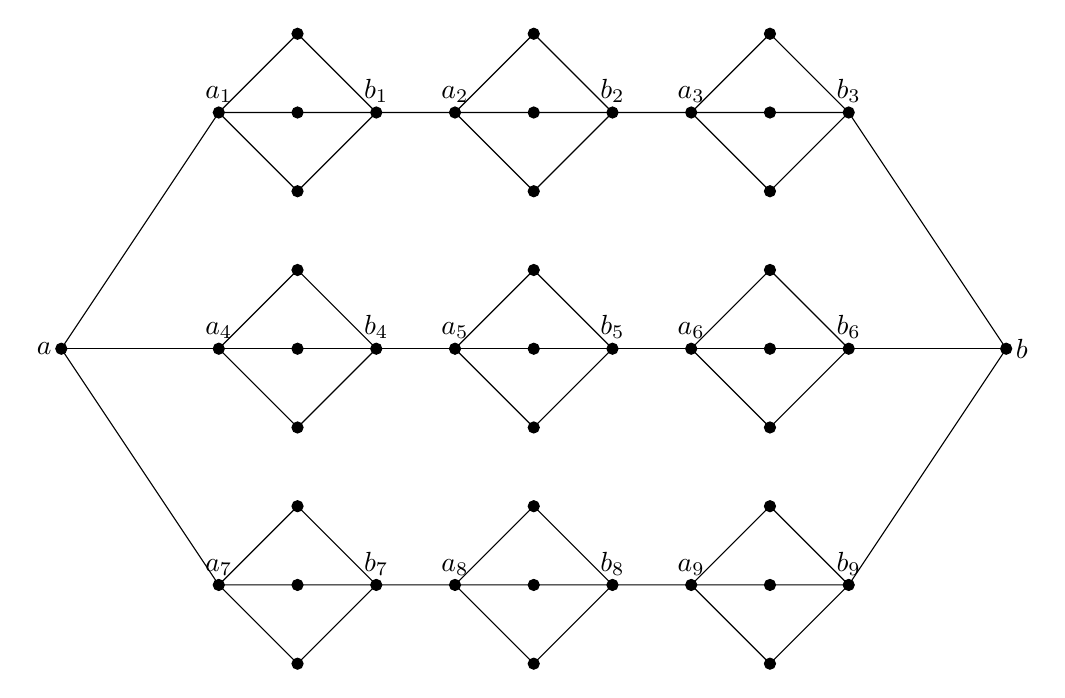
\begin{tikzpicture}

\draw(-6,0)--(6,0);
\filldraw[black](-6,0)node[left]{$a$} circle(2pt);
\filldraw[black](6,0)node[right]{$b$} circle(2pt);
\filldraw[black](-4,3)node[above]{$a_1$} circle(2pt);
\draw(-6,0)--(-4,3)--(4,3)--(6,0);
\draw(-6,0)--(-4,-3)--(4,-3)--(6,0);
\filldraw[black](-1,3)node[above]{$a_2$} circle(2pt);
\filldraw[black](2,3)node[above]{$a_3$} circle(2pt);
\filldraw[black](-4,0)node[above]{$a_4$} circle(2pt);
\filldraw[black](-1,0)node[above]{$a_5$} circle(2pt);
\filldraw[black](2,0)node[above]{$a_6$} circle(2pt);
\filldraw[black](-4,-3)node[above]{$a_7$} circle(2pt);
\filldraw[black](-1,-3)node[above]{$a_8$} circle(2pt);
\filldraw[black](2,-3)node[above]{$a_9$} circle(2pt);
\filldraw[black](-2,3)node[above]{$b_1$} circle(2pt);
\filldraw[black](1,3)node[above]{$b_2$} circle(2pt);
\filldraw[black](4,3)node[above]{$b_3$} circle(2pt);
\filldraw[black](-2,0)node[above]{$b_4$} circle(2pt);
\filldraw[black](1,0)node[above]{$b_5$} circle(2pt);
\filldraw[black](4,0)node[above]{$b_6$} circle(2pt);
\filldraw[black](-2,-3)node[above]{$b_7$} circle(2pt);
\filldraw[black](1,-3)node[above]{$b_8$} circle(2pt);
\filldraw[black](4,-3)node[above]{$b_9$} circle(2pt);
\filldraw[black](-3,4) circle(2pt);
\filldraw[black](-3,3) circle(2pt);
\filldraw[black](-3,2) circle(2pt);
\filldraw[black](-3,1) circle(2pt);
\filldraw[black](-3,0) circle(2pt);
\filldraw[black](-3,-1) circle(2pt);
\filldraw[black](-3,-2) circle(2pt);
\filldraw[black](-3,-3) circle(2pt);
\filldraw[black](-3,-4) circle(2pt);
\filldraw[black](0,4) circle(2pt);
\filldraw[black](0,3) circle(2pt);
\filldraw[black](0,2) circle(2pt);
\filldraw[black](0,1) circle(2pt);
\filldraw[black](0,0) circle(2pt);
\filldraw[black](0,-1) circle(2pt);
\filldraw[black](0,-2) circle(2pt);
\filldraw[black](0,-3) circle(2pt);
\filldraw[black](0,-4) circle(2pt);
\filldraw[black](3,4) circle(2pt);
\filldraw[black](3,3) circle(2pt);
\filldraw[black](3,2) circle(2pt);
\filldraw[black](3,1) circle(2pt);
\filldraw[black](3,0) circle(2pt);
\filldraw[black](3,-1) circle(2pt);
\filldraw[black](3,-2) circle(2pt);
\filldraw[black](3,-3) circle(2pt);
\filldraw[black](3,-4) circle(2pt);
\draw(-4,3)--(-3,4)--(-2,3);
\draw(-4,0)--(-3,1)--(-2,0);
\draw(-4,-3)--(-3,-2)--(-2,-3);
\draw(-4,3)--(-3,2)--(-2,3);
\draw(-4,0)--(-3,-1)--(-2,0);
\draw(-4,-3)--(-3,-4)--(-2,-3);

\draw(-1,3)--(0,4)--(1,3);
\draw(-1,0)--(0,1)--(1,0);
\draw(-1,-3)--(0,-2)--(1,-3);
\draw(-1,3)--(0,2)--(1,3);
\draw(-1,0)--(0,-1)--(1,0);
\draw(-1,-3)--(0,-4)--(1,-3);

\draw(2,3)--(3,4)--(4,3);
\draw(2,0)--(3,1)--(4,0);
\draw(2,-3)--(3,-2)--(4,-3);
\draw(2,3)--(3,2)--(4,3);
\draw(2,0)--(3,-1)--(4,0);
\draw(2,-3)--(3,-4)--(4,-3);




\end{tikzpicture}
\end{center}
\end{figure}


Clearly, the maximum degree of $G$ is $k+1=\Delta$. By Lemma \ref{lm4inbri}, it is not difficult to prove that $G$ does not admit any 2-walk.

\qed







\section{Finding $k$-walks in graphs with lower toughness}
\subsection{Some conjectures on the existence of $k$-trees and $k$-walks}
Recall Theorem \ref{tktree} and Theorem \ref{ktreetokwalk} in Section \ref{sectionktwh}. We have:
$$\frac{1}{k-2}\text{-tough}\Rightarrow k\text{-tree}\Rightarrow k\text{-walk}\Rightarrow\frac{1}{k}\text{-tough}.$$


At the first glance, this chain seems not perfect, since there is a large gap between the head and the tail of the chain. So, can we improve this chain? Do we have the following chain?
$$\frac{1}{k-1}\text{-tough}\Rightarrow k\text{-tree}\Rightarrow k\text{-walk}\Rightarrow\frac{1}{k}\text{-tough}.$$
Or do we have a shorter one?
$$\frac{1}{k-1}\text{-tough}\Rightarrow k\text{-walk}\Rightarrow\frac{1}{k}\text{-tough}.$$
Naturally, Jackson and Wormald posed the following conjecture, which is the main topic of this thesis.
\begin{conjecture}[Jackson, Wormald 1990]\label{mainconjjawo1}
Every $\frac{1}{k-1}$-tough graph admits a $k$-walk.
\end{conjecture}

Similarly, we have another conjecture.
\begin{conjecture}\label{main2ktcon}
Every $\frac{1}{k-1}$-tough graph admits a $k$-tree.
\end{conjecture}

What is more, there is a slight stronger version of this conjecture.

\begin{conjecture}\label{main2strdeli}
For any integer $k\ge2$, if for all $S\subset V(G)$, the number of components in $G-S$, $\Omega(G-S)\le (k-1)|S|+1$, then graph $G$ admits a $k$-tree.
\end{conjecture}

In Conjecture \ref{main2ktcon}, we set $k=2$, then we get:
\begin{conjecture}\label{coj1k1thmilpa}
If graph $G$ is 1-tough, then $G$ admits a Hamilton path, i.e. $G$ is traceable.
\end{conjecture}
Clearly, Theorem \ref{exa2000nh} shows that the conjecture above is false. That means Conjecture \ref{main2ktcon} and Conjecture \ref{main2strdeli} are false when $k=2$. So, it is natural to ask whether they are true when $k\ge3$?

However, the inverse direction of Conjecture \ref{main2strdeli} is true.

\begin{proposition}{\cite[Proposition 5]{ozeki2011spanning}}
For $k\ge2$, if graph $G$ has a $k$-tree, then for all $S\subset V(G)$, $\Omega(G-S)\le(k-1)|S|+1$ and the equality holds if $S$ is an independent set.
\end{proposition}


\begin{proof}
We use mathematical induction. Suppose $T$ is a spanning tree of $G$. If $|S|=0$, there is nothing to prove. Then let us assume $|S|\ge1$. For any $v\in S$, denote $S'=S-\{v\}$. Then by the induction hypothesis, $\Omega(T-S)\le(k-1)|S'|+1$. Denote the component of $T-S'$ containing $v$ by $C$. We observe that $d_C(v)\le d_T(v)\le k$. Obviously, the deletion of $v$ from $C$ divides $C$ into at most $d_C(v)$ components. Therefore:
$$\Omega(T-S)=\Omega(T-S')-1+d_C(v)$$
$$\le(k-1)|S'|+1-1+k$$
$$=(k-1)|S|+1.$$

Thus $\Omega(G-S)\le(k-1)|S|+1.$
\end{proof}





The survey \cite{ozeki2011spanning} is an excellent introduction for the topic of spanning trees, so we strongly recommend readers who are interested in this topic to consult it.

In \cite{ellingham2002connected}, the concept of $k$-trees is generalized into $f(v)$-trees. Thus, Theorem \ref{tktreeslistr2} has the following generalization.
\begin{theorem}[Ellingham, Nam and Voss 2002]\label{tftreeslistr3}
For any connected graph $G$, let $f(v)$ be a positive integer-valued function on $V(G)$. If the number of components $\Omega(G-S)\le\sum_{v\in S}(f(v)-2)+2$ for all $S\subset V(G)$, then $G$ has a spanning tree $T$ with vertex-degree $d_T(v)\le f(v)$ for all $v\in V(G)$.
\end{theorem}

\subsection{Hamilton prisms: the midway between 2-trees and 2-walks}
Let us look at Theorem \ref{ktreetokwalk} again. Clearly, it shows the following chain:
$$\text{1-walk (Hamilton cycle)}\Rightarrow\text{2-tree (Hamilton path)}\Rightarrow\text{2-walk}\Rightarrow\text{3-tree}\Rightarrow\cdots$$
This chain describes a ``natural'' hierarchy for measuring how ``close'' a graph is to being Hamiltonian.

In\cite{kaiser2007hamilton}, Kaiser, Kr{\'a}l, Rosenfeld, Ryj{\'a}{\v c}ed and Voss introduced a conception named {\em Hamilton prisms} which turn out to be a midway between 2-trees and 2-walks.
\begin{definition}
The prism over a graph $G$ is obtained by taking two copies of $G$ and adding a perfect matching joining the two copies of each vertex by an edge.
\end{definition}

It is easy to prove:
\begin{theorem}\label{2thp2wthm1}
~

\begin{enumerate}
\item If a graph $G$ contains a 2-tree, then its prism is Hamiltonian.
\item If  a graph $G$ has a Hamilton prism, then it admits a 2-walk.
\end{enumerate}
\end{theorem}

\begin{proof}
For the first part of the theorem, suppose a graph $G$ contains a Hamilton path (i.e. 2-tree). Take the Hamilton path in each copy and add the two edges necessary to make a Hamilton cycle in the prism.

For the second part, suppose a graph $G$ has a Hamilton prism. Then the 2-walk follows the edges corresponding to the edges in the Hamilton cycle in the prism.
\end{proof}


Please recall Conjecture \ref{4lineh}, in Section \ref{seclandclfg}, which says every 4-connected line graph is Hamiltonian. We know that this conjecture is a famous long-standing conjecture. However, if we lower our expectation, from Hamilton cycles to Hamilton prisms, we see the following result \cite{kaiser2007hamilton}.


\begin{theorem}[Kaiser, Kr{\'a}l, Rosenfeld, Ryj{\'a}{\v c}ed and Voss 2007]\label{2clhpthm1}
For any multigraph $G$, if its line graph $L(G)$ is 2-connected, then the prism over $L(G)$ is Hamiltonian.
\end{theorem}

Recall that Theorem \ref{2to3} tells us that all line graphs are claw-free. So, are all 2-connected claw-free graphs prism-hamiltonian? The answer is affirmative \cite{vcada2004hamiltonian}.


\begin{theorem}[{\v C}ada 2004]\label{2cclwfgphth}
Every 2-connected claw-free graph is prism-hamiltonian.
\end{theorem}

In the research of Hamilton prisms, we also face a conjecture corresponding to the Conjecture \ref{cj1chath}, although a little weaker.

\begin{conjecture}\label{cjttph}
There is a positive constant $t$ such that the prism over every $t$-tough graph is Hamiltonian.
\end{conjecture}

The following theorem plays a similar role with Theorem \ref{exa2000nh}.

\begin{theorem}[Kaiser, Kr{\'a}l, Rosenfeld, Ryj{\'a}{\v c}ed and Voss 2007]\label{98tgnhpex}
There exists a series of graphs $\{G_n\}$ such that each $G_n$ is non-prism-hamiltonian, and the toughness $t(G_n)\rightarrow9/8$, as $n\rightarrow\infty$.
\end{theorem}

\begin{proof}
Here we only describe the structure of the graphs $\{G_n\}$, and omit the detailed proof. The readers interested in this result are recommended to read \cite{kaiser2007hamilton}.

Now, let $A$ stand for the following picture (see Figure \ref{picainv07})
\begin{figure}[h]
\begin{center}
\caption{The graph $A$}\label{picainv07}
\begin{tikzpicture}
\filldraw[black](0,0) circle(2pt);
\filldraw[black](1,1.75)node[above]{$a$} circle(2pt);
\draw(-1,-1.75)--(1,1.75)--(3,-1.75);
\draw(0,0)--(2,0);
\filldraw[black](2,0) circle(2pt);
\filldraw[black](-1,-1.75) circle(2pt);
\filldraw[black](3,-1.75) circle(2pt);
\end{tikzpicture}
\end{center}
\end{figure}

Starting from graph $A$, let us construct the graphs $\{G_n\}$. Now take $4n+1$ vertex-disjoint copies of $A$, namely $A_1,\ldots,A_{4n+1}$, and add all possible edge between the vertices on these copies corresponding to the vertex $a$ in $A$. What is more, add an independent set $U$ of $n$ vertices, and all possible edges between all the vertices of $U$ and all the vertices outside $U$. So, the first graph $G_1$ of this sequence $\{G_n\}$ is like the following picture (see Figure \ref{picg1inv07}).
\begin{figure}[h]
\begin{center}
\caption{The graph $G_1$}\label{picg1inv07}
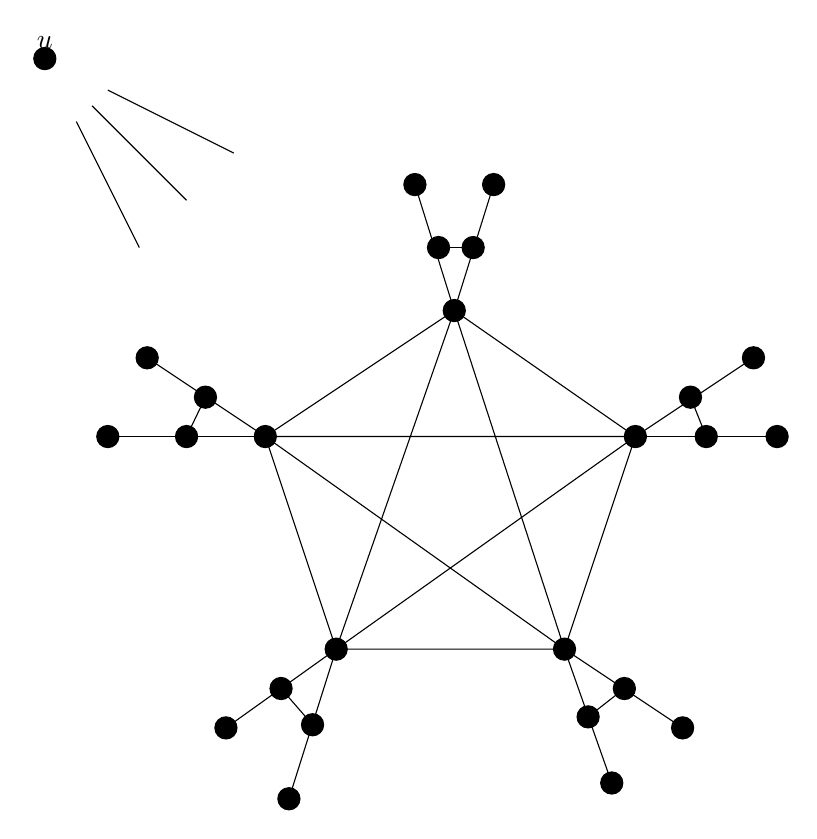
\begin{tikzpicture}[scale=2]
\filldraw[black](2.6,-1.6) circle(2pt);
\filldraw[black](3.75,-2.4) circle(2pt);
\filldraw[black](3.3,-3.75) circle(2pt);
\filldraw[black](1.85,-3.75) circle(2pt);
\filldraw[black](1.4,-2.4) circle(2pt);
\draw(2.6,-1.6)--(3.75,-2.4)--(3.3,-3.75)--(1.85,-3.75)--(1.4,-2.4)--(2.6,-1.6);
\draw(2.6,-1.6)--(3.3,-3.75)--(1.4,-2.4)--(3.75,-2.4)--(1.85,-3.75)--(2.6,-1.6);
\draw(2.6,-1.6)--(2.35,-0.8);
\draw(2.6,-1.6)--(2.85,-0.8);
\filldraw[black](2.5,-1.2) circle(2pt);\filldraw[black](2.72,-1.2) circle(2pt);\draw(2.5,-1.2)--(2.72,-1.2);
\draw(3.75,-2.4)--(4.5,-1.9);
\draw(3.75,-2.4)--(4.65,-2.4);
\filldraw[black](4.1,-2.15) circle(2pt);\filldraw[black](4.2,-2.4) circle(2pt);\draw(4.1,-2.15)--(4.2,-2.4);
\draw(3.3,-3.75)--(3.6,-4.6);
\draw(3.3,-3.75)--(4.05,-4.25);
\filldraw[black](3.45,-4.18) circle(2pt);\filldraw[black](3.68,-4) circle(2pt);\draw(3.45,-4.18)--(3.68,-4);
\draw(1.85,-3.75)--(1.15,-4.25);
\draw(1.85,-3.75)--(1.55,-4.7);
\filldraw[black](1.5,-4) circle(2pt);\filldraw[black](1.7,-4.23) circle(2pt);\draw(1.5,-4)--(1.7,-4.23);
\draw(1.4,-2.4)--(0.65,-1.9);
\draw(1.4,-2.4)--(0.4,-2.4);
\filldraw[black](1.02,-2.15) circle(2pt);\filldraw[black](0.9,-2.4) circle(2pt);\draw(1.02,-2.15)--(0.9,-2.4);
\filldraw[black](2.35,-0.8) circle(2pt);
\filldraw[black](2.85,-0.8) circle(2pt);
\filldraw[black](4.5,-1.9) circle(2pt);
\filldraw[black](4.65,-2.4) circle(2pt);
\filldraw[black](3.6,-4.6) circle(2pt);
\filldraw[black](4.05,-4.25) circle(2pt);
\filldraw[black](1.15,-4.25) circle(2pt);
\filldraw[black](1.55,-4.7) circle(2pt);
\filldraw[black](0.65,-1.9) circle(2pt);
\filldraw[black](0.4,-2.4) circle(2pt);
\filldraw[black](0,0)node[above]{$u$} circle(2pt);
\draw(0.4,-0.2)--(1.2,-0.6);
\draw(0.3,-0.3)--(0.9,-0.9);
\draw(0.2,-0.4)--(0.6,-1.2);
\end{tikzpicture}
\end{center}
\end{figure}

\end{proof}
\newpage
In the end of this section, let us look at a result \cite{kral2007closure}, which might be considered as an analogue of Theorem \ref{thmcloham1}.

\begin{theorem}[Kr{\'a}l, Stacho 2007]\label{cloprihth2}
For any graph $G$ with $n$ vertices, let $x$ and $y$ be two non-adjacent vertices such that the sum of their degree is at least $4n/3-4/3$. Then $G$ has a Hamilton prism if and only if $G+xy$ does.

\end{theorem}


















\section{From edge-dominating cycles to $k$-walks}

The central task of this thesis is to prove that Conjecture \ref{mainconjjawo1} holds for $2K_2$-free graphs, and the $k$-walks can be found in time polynomial on $|V(G)|$. The proof is divided into two parts. First, we shall prove that if a graph $G$ admits an edge-dominating cycle, then Conjecture \ref{mainconjjawo1} holds for this graph. Second, we shall prove that every $2K_2$-free graph, who is not a tree, admits an edge-dominating cycle, which can be found in polynomial time.

In this section, we focus on the following theorem \cite{gao2015on}.


\begin{theorem}[Gao, Pasechnik 2015]\label{mthm1}
If $G$ has an edge-dominating cycle and if $G$ is $\frac{1}{k-1}$-tough, then $G$ admits a $k$-walk.
\end{theorem}

\begin{proof}
Denote the edge-dominating cycle as $C$, thus the induced subgraph $D=G-C$ is a coclique. For any subset $D_0\subset D$, by $\frac{1}{k-1}$-toughness, $D_0$ has at least $\lceil\frac{|D_0|}{k-1}\rceil$ neighbors in $C$. By  Theorem \ref{zuiqianghallt}, there is $E'\subset E(G)$ such that each $e\in E'$ has one vertex in $D$ and the other in $C$. And each vertex in $D$ is incident to exactly one edge in $E'$, while each vertex in $C$ is incident to at most $k-1$ edges in $E'$. Then these (doubled) edges in $E'$ and the edges in the edge-dominating cycle $C$ form a $k$-walk in $G$.
\end{proof}






\section{From edge-dominating cycles to Hamilton prisms}
As we have seen, edge-dominating cycles have a powerful implication in finding $k$-walks. Since the concept of Hamilton prisms is an analogy of the concept of $k$-walks, so we can expect that edge-dominating cycles have similar applications on finding Hamilton prisms. Indeed, we obtain the following result.
\begin{theorem}[Gao, Pasechnik 2015]\label{edhctohprthlm}
Suppose $G$ is $(1+\epsilon)$-tough, for some $\epsilon>0$.
\begin{enumerate}
\item If $G$ contains an edge-dominating cycle $C$ with even number of vertices, then the prism of $G$ is Hamiltonian.
\item If $G$ contains an edge-dominating cycle $C=v_1v_2\cdots v_{2p+1}v_1$ of odd length, and there are three vertices $v_1$, $v_{2q}$ and $v_{2q+1}$, for some $0\le q\le p$, inducing a triangle in $G$, then the prism over $G$ is Hamiltonian.
\end{enumerate}
\end{theorem}

\begin{proof}
For the first part (see the following picture), denote the (even size) edge-dominating path in $G$ by $C=v_1v_2\cdots v_{2p}v_1$. The set of vertices outside the path $D=V(G)-V(C)$ is an independent set. By Hall's Theorem and 1-toughness, there is a matching $M$, from $D$ to $C$. That means for any vertex $u_j$ in $D$, there is a vertex $v_{i_j}$ on $C$ adjacent to $u_j$ in $M$.

Obviously, we have a Hamilton cycle in $\bar{C}$, the prism over $C$, namely $$v_1v'_1v'_2v_2\cdots v_{2p-1}v'_{2p-1}v'_{2p}v_{2p}v_1.$$ Now, we change every  $v_{i_j}v'_{i_j}$ (or $v'_{i_j}v_{i_j}$) into $v_{i_j}u_ju'_jv'_{i_j}$ (or $v'_{i_j}u'_ju_jv_{i_j}$) to get a Hamilton cycle in $\bar{G}$.

\begin{figure}[h]
\caption{$G$ has an edge-dominating cycle of even length}
\begin{center}
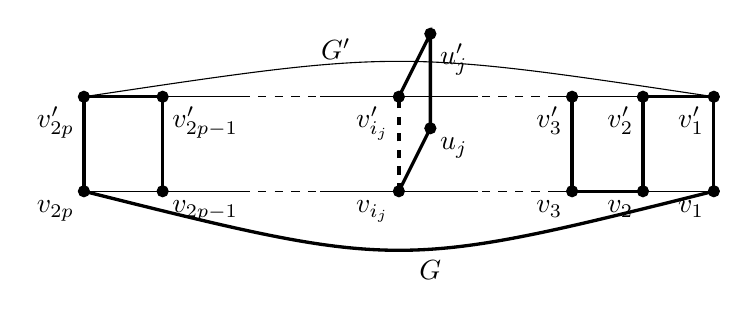
\begin{tikzpicture}[scale=2]
\draw(-2,0)node[below left]{$v_{2p}$}--(-1,0);\draw(-0.5,0)--(0.5,0);\draw(1,0)--(2,0);
\draw(-2,0.6)node[below left]{$v'_{2p}$}--(-1,0.6);\draw(-0.5,0.6)--(0.5,0.6);\draw(1,0.6)--(2,0.6);
\filldraw[black](0,0)node[below left]{$v_{i_j}$} circle(1pt);
\filldraw[black](0,0.6)node[below left]{$v'_{i_j}$} circle(1pt);
\filldraw[black](-2,0.6) circle(1pt);
\filldraw[black](2,0.6)node[below left]{$v'_1$} circle(1pt);
\filldraw[black](-1.5,0.6)node[below right]{$v'_{2p-1}$} circle(1pt);
\filldraw[black](1.55,0.6)node[below left]{$v'_2$} circle(1pt);
\filldraw[black](2,0)node[below left]{$v_1$} circle(1pt);
\filldraw[black](-2,0) circle(1pt);
\filldraw[black](1.55,0)node[below left]{$v_2$} circle(1pt);
\filldraw[black](-1.5,0)node[below right]{$v_{2p-1}$} circle(1pt);
\draw[dashed](-1,0)--(-0.5,0);
\draw[dashed](1,0)--(0.5,0);
\draw[dashed](-1,0.6)--(-0.5,0.6);
\draw[dashed](1,0.6)--(0.5,0.6);
\filldraw[black](1.1,0)node[below left]{$v_3$} circle(1pt);
\filldraw[black](1.1,0.6)node[below left]{$v'_3$} circle(1pt);
\filldraw[black](0.2,0.4)node[below right]{$u_j$} circle(1pt);
\filldraw[black](0.2,1)node[below right]{$u'_j$} circle(1pt);
\draw[very thick](2,0)--(2,0.6)--(1.55,0.6)--(1.55,0)--(1.1,0)--(1.1,0.6);
\draw[very thick](0,0)--(0.2,0.4)--(0.2,1)--(0,0.6);
\draw[dashed, very thick](0,0)--(0,0.6);
\draw[very thick](-1.5,0)--(-1.5,0.6)--(-2,0.6)--(-2,0);
\draw[very thick](-2,0)..controls(0,-0.5)..(2,0);
\draw(-2,0.6)..controls(0,0.9)..(2,0.6);
\node at(0.2,-0.5){$G$};\node at (-0.4,0.9){$G'$};
\end{tikzpicture}

\end{center}
\end{figure}


For the second part, denote the (odd length) edge-dominating cycle in $G$ by $C=v_1v_2\cdot v_{2p+1}v_1$ (see Figure \ref{fig2}). The set of vertices outside the cycle $D=V(G)-V(C)$ is an independent set. By Hall's Theorem, and $(1+\epsilon)$-tough, there is a matching $M$ from $D$ to $C-\{v_1\}$. That means for any vertex $u_j$ in $D$, there is a vertex $v_{i_j}$ on $C-\{v_1\}$ adjacnet to $u_j$ in $M$.

Clearly, we have a Hamilton cycle in $\bar{C}$, namely $$v_1v_2v'_2v'_3v_3\cdots v_{2q-1}v_{2q}v'_{2q}v'_1v'_{2q+1}v_{2q+1}\cdots v_{2p+1}v_1.$$
Now, we change every  $v_{i_j}v'_{i_j}$ (or $v'_{i_j}v_{i_j}$) into $v_{i_j}u_ju'_jv'_{i_j}$ (or $v'_{i_j}u'_ju_jv_{i_j}$) to get a Hamilton cycle in $\bar{G}$.

\begin{figure}[h]
\caption{$G$ has an edge-dominating cycle of odd length}\label{fig2}
\begin{center}
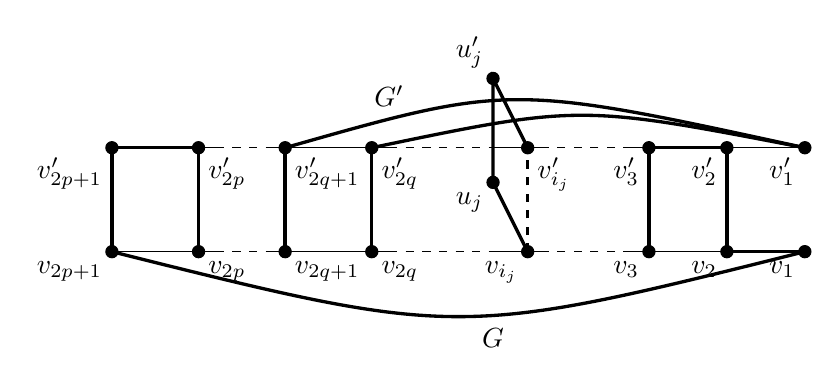
\begin{tikzpicture}[scale=2.2]
\draw(-2,0)node[below left]{$v_{2p+1}$}--(-1.4,0);\draw(1,0)--(2,0);
\draw(-2,0.6)node[below left]{$v'_{2p+1}$}--(-1.4,0.6);\draw(1,0.6)--(2,0.6);
\filldraw[black](0.4,0)node[below left]{$v_{i_j}$} circle(1pt);
\filldraw[black](0.4,0.6)node[below right]{$v'_{i_j}$} circle(1pt);
\filldraw[black](-2,0.6) circle(1pt);
\filldraw[black](2,0.6)node[below left]{$v'_1$} circle(1pt);
\filldraw[black](-1.5,0.6)node[below right]{$v'_{2p}$} circle(1pt);
\filldraw[black](1.55,0.6)node[below left]{$v'_2$} circle(1pt);
\filldraw[black](2,0)node[below left]{$v_1$} circle(1pt);
\filldraw[black](-2,0) circle(1pt);
\filldraw[black](1.55,0)node[below left]{$v_2$} circle(1pt);
\filldraw[black](-1.5,0)node[below right]{$v_{2p}$} circle(1pt);
\draw[dashed](-1.4,0)--(-1.1,0);\draw(-1.1,0)--(-0.4,0);\filldraw[black](-1,0)node[below right]{$v_{2q+1}$} circle(1pt);
\draw[dashed](1,0)--(0.5,0);
\draw[dashed](-1.4,0.6)--(-1.1,0.6);\draw(-1.1,0.6)--(-0.4,0.6);\filldraw[black](-1,0.6)node[below right]{$v'_{2q+1}$} circle(1pt);
\draw[dashed](1,0.6)--(0.5,0.6);
\filldraw[black](1.1,0)node[below left]{$v_3$} circle(1pt);
\filldraw[black](1.1,0.6)node[below left]{$v'_3$} circle(1pt);
\filldraw[black](0.2,0.4)node[below left]{$u_j$} circle(1pt);
\filldraw[black](0.2,1)node[above left]{$u'_j$} circle(1pt);
\draw[very thick](2,0)--(1.55,0)--(1.55,0.6)--(1.1,0.6)--(1.1,0);
\draw[very thick](0.4,0)--(0.2,0.4)--(0.2,1)--(0.4,0.6);
\draw[dashed, very thick](0.4,0)--(0.4,0.6);
\draw[very thick](-1.5,0)--(-1.5,0.6)--(-2,0.6)--(-2,0);
\draw[very thick](-2,0)..controls(0,-0.5)..(2,0);

\node at(0.2,-0.5){$G$};\node at (-0.4,0.9){$G'$};
\draw[dashed](-0.4,0)--(0.2,0);\draw(0.2,0)--(0.5,0);
\draw[dashed](-0.4,0.6)--(0.2,0.6);\draw(0.2,0.6)--(0.5,0.6);
\filldraw[black](-0.5,0)node[below right]{$v_{2q}$} circle(1pt);
\filldraw[black](-0.5,0.6)node[below right]{$v'_{2q}$} circle(1pt);
\draw[very thick](-0.5,0.6)..controls(0.7,0.85)..(2,0.6);
\draw[very thick](-1,0.6)..controls(0.3,0.97)..(2,0.6);
\draw[very thick](-0.5,0.6)--(-0.5,0);
\draw[very thick](-1,0.6)--(-1,0);

\end{tikzpicture}

\end{center}
\end{figure}


\end{proof}












































\newpage

\section{2-walks in some special graphs}

\subsection{General cases}
Recall that Theorem \ref{tktree} and Theorem \ref{ktreetokwalk} tell us  for every integer $k\ge3$, every $\frac{1}{k-2}$ graph admits a $k$-walk. On the other hand, we have already known many results on the existence of Hamilton cycles (1-walks). So, what happens in the gap, on 2-walks?

In \cite{ellingham2000toughness}, Ellingham and Zha proved the following remarkable result.

\begin{theorem}[Ellingham, Zha 2000]\label{4thgrhhas2w}
Every 4-tough graph admits a 2-walk.
\end{theorem}

In fact, they proved an even stronger result.
\begin{theorem}[Ellingham, Zha 2000]\label{4thgrhhas2wdet}
For any subset of vertices in graph $G$, $S\subset V(G)$ with $\Omega(G-S)\ge2$, if $\Omega(G-S)\le\min\{|S|/2,(|S|+9)/4\}$ is always true, then $G$ contains a 2-walk.
\end{theorem}

The proof of Theorem \ref{4thgrhhas2wdet} uses a concept called {\em quasitrees}.

\subsubsection{Toughness and quasitrees}
For any graph $G$, suppose $F$ is a spanning subgraph (possibly disconnected). Color the edges of $G$ in the following way: edges in $F$ or joining two vertices in the same component are red, and all edges connecting two vertices in different components of $F$ are green. Then, a {\em quasitree} (derived from) in $G$ is a connected subgraph of $G$ that is the union of $i$ components of $F$ and $i-1$ green edges whose endpoints are in these components, for some $i\ge1$. For any $k\ge1$ and a subgraph $H$ of $G$, a $k$-quasitree for $H$ is a quasitree in $G$ which is a spanning subgraph of $H$ and in which each vertex is incident to at most $k$ green edges.

The following lemmas are useful in the proof of Theorem \ref{4thgrhhas2wdet}.

\begin{lemma}[Ellingham, Zha 2000]\label{lm31inez}
For any integer $k\ge1$, $g\ge1$, suppose $Q$ is a $k$-quasitree derived from $F$, where each component of $F$ contains at least $g$ vertices. If $S$ is a nonempty set of vertices of quasidegree (the number of green edges incident to the vertex) $k$ in $Q$. Then:
\begin{enumerate}
\item $\Omega(Q-S)\ge(k-2)|S|+2$ if $g=1$,
\item $\Omega(Q-S)\ge(k-1)|S|+2$ if $g\ge2$.
\end{enumerate}
\end{lemma}


\begin{lemma}[Ellingham, Zha 2000]\label{lm32inez}
Let $Q$ be a quasitree and $R$ a nonempty set of green edges of $Q$. Then for any $q\ge2$, the number of components in $Q-R$ which are incident in $Q$ with less than $q$ edges of $R$ is at least $(q-2)|R|/(q-1)+q/(q-1)$. 
\end{lemma}


\begin{lemma}[Ellingham, Zha 2000]\label{lm33inez}
Assume $g\ge2$ and $Q$ is a quasitree derived from $F$, with each component having at least $g$ vertices. If $S$ is a nonempty set of vertices of quasidegree 1 in $Q$, then $\Omega(Q-S)\ge\frac{(g-2)|S|}{2(g-1)}+\frac{g}{g-1}$.
\end{lemma}

With the help of these lemmas above, Ellingham and Zha proved the following theorem on the existence of quasitrees.

\begin{theorem}[Ellingham, Zha 2000]\label{thm35inez}
For any positive integers $g$ and $k$ with $g+k\ge3$, suppose that $G$ is a connected graph with a spanning subgraph $F$, each component of which has order at least $g$ and for each $S\subset V(G)$, we have:
\begin{enumerate}
\item $\Omega(G-S)<\frac{(g-2)|S|}{2(g-1)}+\frac{2g-1}{g-1}$ if $k=1$ and $g\ge2$, or
\item $\Omega(G-S)<(k-2)|S|+3$ if $k\ge2$ and $g=1$, or
\item $\Omega(G-S)<(k-1)|S|+3$ if $k\ge2$ and $g\ge2$.
\end{enumerate}
Then $G$ contains a $k$-quasitree derived from $F$.
\end{theorem}










\subsubsection{The proof of Theorem \ref{4thgrhhas2wdet} (Ellingham, Zha 2000)}

From the assumption $\Omega(G-S)\le\min\{|S|/2,(|S|+9)/4\}$, we know that $G$ is 2-tough, and obviously $G$ is connected as well. By Corollary \ref{kttokfejks}, $G$ contains a 2-factor $F$. Again, we have $\Omega(G-S)\le(|S|+9)/4<|S|/4+5/2$. By Theorem \ref{thm35inez}, with $g=3$ and $k=1$, we know that $G$ contains a 1-quasitree $Q$ derived from $F$. Now doubling each green edge of $Q$, we get an Euler multigraph in which each vertex has degree 2 or 4. Clearly, this closed Euler trail in this multigraph corresponding to a 2-walk in $G$. \qed











\subsection{Circuit graphs}
The definition of {\em circuit graphs} was first given by Barnette in \cite{barnette1966trees}, as following.
\begin{definition}
For any 3-polyhedral graph $G$, who is embedded in the plane $\Pi$, let $J$ be a simple circuit of $G$, and let $G(J)$ denote the graph consisting of $J$ together with all vertices and edges of $G$ that are interior to the region of plane bounded by $J$. Then $G(J)$ is called a circuit graph and the edges of $G(J)$ who are not on $J$ are called interior edges.
\end{definition}
Here a graph $G$ is called {\em 3-polyhedral (or $d$-polyhedral)}, if $G$ is isomorphic to the graph formed by vertices and edges of a 3-dimensional (or $d$-dimensional) bound convex polyhedron.

\begin{proposition}
A graph $G$ is 3-polyhedral if and only if $G$ is a 3-connected planar graph.
\end{proposition}

In \cite{barnette1966trees}, Barnette proved:

\begin{theorem}[Barnette 1966]\label{3cp3tthm66}
Every 3-polyhedral graph $G$ admits a 3-tree.
\end{theorem}

As we have seen in Theorem \ref{ktreetokwalk}, admiting a 3-tree is a stronger condition than having a 3-walk, but weaker than having 2-walk.
Obviously, every 3-polyhedral graph is a circuit graph. So, is Theorem \ref{3cp3tthm66} still true for circuit graphs? The answer is affirmative. What is more, Z. Gao and R. Richter \cite{gao19942} proved a slight stronger result.

\begin{theorem}[Z. Gao, R. Richter]\label{2wincgthm941}
Every circuit graph admits a 2-walk.

\end{theorem}

To prove this theorem, they introduced an equivalent definition for circuit graphs.
\begin{definition}
A circuit graph is an ordered pair $(G,C)$ such that:
\begin{enumerate}
\item $G$ is a 2-connected graph and $C$ is a polygon in $G$.
\item There is an embedding of $G$ in the plane such that $C$ bounds a face.
\item If $(H,K)$ is a 2-seperation of $G$, then $C\not\subset H$ and $C\not\subset K$.
\end{enumerate}
\end{definition}

Here, for a graph $G$, a {\em $k$-seperation} is a pair $(H,K)$ of subgraphs of $G$ such that $G=H\cup K$, and $H\cap K$ is an independent set of vertices in $G$, and both $H$ and $K$ have at least $k$ edges.
\begin{proposition}
A graph $G$ is $n$-connected if and only if $G$ has more than $n$ vertices while no $k$ seperation for any $0\le k<n$.
\end{proposition}

Specifically, in \cite{gao19942}, they proved the following version of Theorem \ref{2wincgthm941}.

\begin{theorem}[Z. Gao, R. Richter]\label{2wincgde942}
For any circuit graph $(G,C)$, suppose $x$ and $y$ are two different vertices on $C$, and let $\vec{C}$ be a orientation of $C$, then there exists a closed walk $W$ such that:
\begin{enumerate}
\item $W$ visits each vertex in $G$ either once or twice.
\item $W$ visits each of $x$ and $y$ exactly once.
\item $W$ uses each edge in $C$ exactly once and the direction of $W$ agree with $\vec{C}$.
\end{enumerate}
\end{theorem}









\subsection{$K_4$-minor-free graphs}
In the last section, we have seen an example on the existence of 2-walks in some special graphs. However, we did not use any condition on toughness. So, in this section, we look at an example of finding 2-walks under the assumption of some toughness requirement.

In \cite{dvovrak2010toughness}, Dvo{\v r}{\'a}k, Kr{\'a}l and Teska proved the following theorem on the existence of 2-walks for $k_4$-minor-free graphs.
\begin{theorem}[Dvo{\v r}{\'a}k, Kr{\'a}l and Teska 2010]\label{thmk4mfg2w}
If $K_4$-minor-free graph $G$ is more than $4/7$-tough, then $G$ admits a 2-walk.
\end{theorem}

Obviously, if $G$ does not has $K_4$ as a minor, then $G$ has neither $K_5$ nor $K_{3,3}$ as a minor. So, by Theorem \ref{plgfodmthmku}, $G$ is a planar graph.

Since the proof of Theorem \ref{thmk4mfg2w} is very tricky, so we do not include it in this here. And we recommend readers who are interested in this topic to consult \cite{dvovrak2010toughness} for the detailed proof.

Additionally, Dvo{\v r}{\'a}k, Kr{\'a}l and Teska also pointed out that Theorem \ref{thmk4mfg2w} is best possible, by constrcuting an example, in the following sense:
\begin{theorem}[Dvo{\v r}{\'a}k, Kr{\'a}l and Teska 2010]\label{cedkt10thm2}
There exists a $4/7$-tough $K_4$-minor-free graph who admits no 2-walk.
\end{theorem}

In fact, their example is also chordal. And in the following section, we shall investigate the conditions for chordal planar graphs to have 2-walks.







\subsection{Chordal planar graphs}

In this section, let us come back to a class graphs which we are familiar with, the chordal planar graphs. Recall that Theorem \ref{plch} in Section \ref{secchoginht} tells us every chordal planar graph with toughness larger than 1 has a Hamilton cycle (1-walk). On the other hand, Theorem \ref{cedkt10thm2} in last section provides an example of $4/7$-tough chordal planar graph having no 2-walk. So, we can expect a number $4/7\le t\le1$ such that every (larger than) $t$-tough chordal planar graph contains a 2-walk.

In \cite{teska20092}, Teska found such a $t$.
\begin{theorem}[Teska 2009]\label{thm34t2w1}
If chordal planar graph $G$ has toughness $t(G)>3/4$, then $G$ contains a 2-walk.
\end{theorem}


\subsubsection{The outline of the proof of Theorem \ref{thm34t2w1}}
To begin with, let us recall Proposition \ref{pdir61}, \ref{c2.2} and \ref{c2.3} on chordal graphs.

Generally, speaking, the proof of Theorem \ref{thm34t2w1} is by mathematical induction. The proof is divided into three steps, each step corresponds to a lemma in the following.

\begin{lemma}[Teska 2009]\label{lm21intes09}
In any 2-connected chordal planar graph $G$, there exists a sequence of subgraphs $G_0,\ldots,G_k$ and a sequence of sets of vertices $S_0,\ldots,S_{k-1}$ such that:
\begin{enumerate}
\item $G_0=K_3$, the triangle.
\item $V(G_{i+1})=V(G_i)\cup S_i$, where $S_i\cap V(G_i)=\emptyset$, the induced subgraph on $V(G_i)$ of $G_{i+1}$ is exactly $G_i$, $N_{G_{i+1}}(S_i)\subset V(G_i)$ and for each $x\in S_i$, the induced subgraph of $G_{i+1}$ on $N_{G_{i+1}}(x)$ is complete for $i=0,1,\ldots,k-1$.
\item $G_k=G$.
\item The integer $k$, the subgraphs $G_i$ $(i=0,\ldots,k)$ and the sets $S_i$ $(i=0,\ldots,k-1)$ can be chosen such that for each $i=0,\ldots,k-1$
\begin{enumerate}
\item there exist a vertex $v_i\in V(G_i)$ so that $v_i$ is simplicial in $G_i$ and $S_i\subset N_{G_{i+1}}(v_i)$;
\item if $x\in S_i$ has degree $d_{G_{i+1}}(x)=3$, then $x$ lies in the inner face of the induced subgraph of $G_{i+1}$ on $N_{G_{i+1}}(x)$.
\end{enumerate}
\end{enumerate}
\end{lemma}

The proof of this lemma is quite thicky, so we omit it here. We recommend the readers who are interested in this topic to consult \cite{teska20092} for the details.

For a 2-connected chordal planar graph  $G$, let $G_0,\ldots,G_k$ and $S_0,\ldots,S_{k-1}$ be any sequences of subgraphs and sets described above. We say the sequence $(G_0,\ldots,G_k;S_0,\ldots,S_{k-1})$ is a {\em convenient construction} of $G$ and for any $x\in S_i$, $i=0,\ldots,k-1$, a vertex $v_i$ with the properties given  above is said to be a parent of the vertex $x$, denoted by $v_i=p(x)$. 

\begin{lemma}[Teska 2009]\label{lm22intes09}
If $(G_0,\ldots,G_k;S_0,\ldots,S_{k-1})$ is a convenient construction, as defined above, of a $t$-tough chordal planar graph $G$, then every graph $G_i$, for $0\le i\le k-1$, is also $t$-tough.
\end{lemma}

\begin{proof}
For any subgraph $G_i$ from the convenient construction with $0<j\le k$, if there exists a set of vertex $P$ such that $\Omega(G_i-P)<\Omega(G_{j-1}-P)$, then there exist two components $C_1$, $C_2$ of $G_{i-1}-P$ so that both $C_1$ and $C_2$ are in the same component of $G_i-P$. We get $G_i$ by adding new simplical vertices to $G_{j-1}$. There must be a simplicial vertex $v$ in $G_j$ who has two neighbors $v_1$, $v_2$ so that $v_1\in C_1$ and $v_2\in C_2$. This is a contradiction since $v_1$ is not adjacent to $v_2$, which contradicts with the fact $v$ is simplicial.
\end{proof}

In the next lemma, we need a concept {\em good 2-walk}, we recommend readers to look up \cite[Lemma 2.2 and 2.3]{teska20092} for this definition.
\begin{lemma}[Teska 2009]\label{lm23intes09}
For any chordal planar graph $G$ with toughness larger than $3/4$, let $G_0,\ldots,G_r;S_0,\ldots,S_{r-1})$ be a  convenient construction of $G$. If for some $i$, with $0\le i\le r-1$, all graphs $G_l$ have good 2-walk $T_l$, for $l=\{0,\ldots,i\}$, then the graph $G_{i+1}$ contains a good 2-walk $T_{i+1}$. 
\end{lemma}
The proof of this lemma is quite long, so we omit it here, and we recommend readers who are interested in this to read \cite{teska20092}.

Finally, because $K_3$ certainly contains a 2-walk, then by Lemma \ref{lm21intes09}, \ref{lm22intes09} and \ref{lm23intes09}, we finish the proof of Theorem \ref{thm34t2w1}
\qed

\subsection{Triangle-free graphs}
In this section, let us look at an application of Theorem \ref{mthm1} on triangle-free graphs. Obviously, by Theorem \ref{mthm1}, the key point for finding a 2-walk is to find an edge-dominating cycle. The following three lemmas come from \cite{aung1989longest}, \cite{bauer2008long} and \cite{ozeki2011dominating}.


\begin{lemma}\cite[Corollary 1.4]{aung1989longest}\label{lmflcitfg1th}
Suppose $G$ is a 2-connected triangle-free graph. If $$\delta(G)\ge\frac{|G|}{6}+1,$$ then $G$ contains an edge-dominating cycle.
\end{lemma}

\begin{lemma}\cite[Theorem 1.7]{bauer2008long}\label{lmt17lci2tfg}
Suppose $G$ is a 2-connected triangle-free graph, and $c(G)$ stands for the circumference of $G$ as usual. If $$c(G)<\min\{|V(G)|,4\delta(G)-4\},$$ then every longest cycle in $G$ is edge-dominating.
\end{lemma}


\begin{lemma}\cite[Theorem 6]{ozeki2011dominating}\label{lmth6indcitfg1}
Suppose $G$ is a 2-connected triangle-free graph. If $$\alpha(G)\le2\kappa(G)-1,$$ then $G$ contains a longest cycle which is also edge-dominating.
\end{lemma}

Now, combine Lemma \ref{lmflcitfg1th}, Lemma \ref{lmt17lci2tfg}, Lemma \ref{lmth6indcitfg1}, Proposition \ref{prokg2t} and Theorem \ref{mthm1}, we get the following results on the existence of 2-walks in 1-tough triangle-free graphs.

\begin{theorem}\label{co2wintfgdelg61}
Suppose $G$ is a 1-tough triangle-free graph. If $$\delta(G)\ge\frac{|G|}{6}+1,$$ then $G$ admits a 2-walk.
\end{theorem}

\begin{theorem}\label{co2wtfgcir}
Suppose $G$ is a 1-tough triangle-free graph, and $c(G)$ stands for the circumference of $G$ as usual. If $$c(G)<\min\{|V(G)|,4\delta(G)-4\},$$ then $G$ admits a 2-walk.
\end{theorem}

\begin{theorem}\label{co2wrfgalpka}
Suppose $G$ is a 1-tough triangle-free graph. If $$\alpha(G)\le2\kappa(G)-1,$$ then $G$ admits a 2-walk.
\end{theorem}















\chapter{$2K_2$-free graphs}\label{chap2k2fg}
In this chapter, we shall introduce another main result in this thesis, proving that every $\frac{1}{k-1}$-tough $2K_2$-free graph $G$ admits a $k$ walk, which can be found in time polynomial to $|V(G)|$.

In the first two sections, we investigate the structural properties of $2K_2$-free graphs and the relation between $2K_2$-free graphs and split graphs. In section \ref{sec53h2k2}, we introduce a recent result, by Broersma, Patel and Pyatkin, that every 25-tough $2K_2$-free graph admits a Hamilton cycle. In section \ref{sec54kw2k2}, we prove Jackson-Wormald's Conjecture for $2K_2$-free graphs. In Section \ref{sec55hpo2}, we investigate the existence of Hamilton prisms in $2K_2$-free graphs. In the last two sections, we discuss some further properties, generalizations and conjectures related with $2K_2$-free graphs.

A {\em $2K_2$-free graph} $G$ is a graph contains no induced subgraph consisting two vertex-disjoint edges. The following observations are obvious.
\begin{proposition}
Suppose $G$ is a $2K_2$-free graph, if $G$ contains no isolated vertex, then $G$ is connected,

\end{proposition}

\begin{proposition}\label{ob1inbro14}
A graph $G$ is a $2K_2$-free graph if and only if for any $A\subset V(G)$, there is at most one component of the induced subgraph $G-A$ contains edges.
\end{proposition}
\section{The structural properties of $2K_2$-free graphs}
In this section, we list several fundamental properties of $2K_2$-free graphs, which are important in our research. Most of these result come from \cite{chung1990maximum} and \cite{broersma2014toughness}.


In \cite{chung1990maximum}, Chung, Gy{\'a}rf{\'a}s, Tuza and Trotter proved several structural theorems for $2K_2$-free graphs while they were studying on extremal graphs.

\begin{theorem}[Chung, Gy{\'a}rf{\'a}s, Tuza and Trotter 1990]\label{str2k2thm1chu90}
For any $2K_2$-free graph $G$, if the clique number $\omega(G)\ge3$, then $G$ contains a dominating clique of size $\omega(G)$.
\end{theorem}

\begin{proof}
As the assumption, we have $p=\omega(G)\ge3$. Let us arbitrarily choose a $p$-element clique, say $K=\{x_1,\ldots,x_p\}$, from $G$, such that $t=|V(G)-Dom(K)|$ is minimum (here $Dom(K)=K\cup N(K)$).

If $t=0$, $K$ is already dominating, there is nothing to prove. Now we consider the case $t>0$. Denote $Z=V(G)-Dom(K)$. Because $p\ge2$, $Z$ is an independent set. Otherwise, an edge in $Z$ and an edge in $K$ form a $2K_2$. For any $i=1,2,\ldots,p$, let $Y_i=\{y\in Dom(K):yx_i\in E(G)\text{ if and only if}i=j$. Because $p\ge3$, every $Y_i$ is an independent set.

Now, arbitrarily choose an element $z_0\in Z$ and let $y_0\in Dom(K)$ be any neighbor of $z_0$. Because $G$ is $2K_2$-free and $p$ is maximal, there exists a unique $i\le p$ such that $y_0x_j\in E(G)$ if and only if $i\neq j$. Thus $K'=(K-\{x_i\})\cup\{y_0\}$ is a clique of size $p$. What is more, each vertex dominated by $K$ is also dominated by $K'$ except possibly those vertices in the set $Y'_i=\{y\in Y_i:y_0y\not\in E(G)\}$. Because $z_0\in Dom(K')$, the minimality of $t$ requires that $Y'_i\neq\emptyset$. Let $y_1\in Y'_i$. Then the edge $z_0y_0$ and $x_iy_1$  force $z_0y_1\in E(G)$. Then choose different $j,k\in\{1,\ldots,p\}-\{i\}$, we get that $z_0y_1$ and $x_ix_k$ are vertex-disjoint edges. Contradiction.
\end{proof}
Using a similar method, we can prove the following generalization.
\begin{theorem}\label{thmcormaldomclitrf}
For any $2K_2$-free graph $G$ with clique number $\omega(G)\ge3$, if $K$ is a maximal (not necessarily maximum) clique, then $K$ is dominating in $G$.
\end{theorem}


\subsection{Triangle-free, $2K_2$-free graphs}\label{sec511}
The following result was first discovered by Chung, Tuza and Trotter in \cite{chung1990maximum}. And in \cite{broersma2014toughness}, Broersma, Patel and Pyatkin proved it again. 

\begin{theorem}[Chung, Tuza and Trotter 1990]\label{thmkindtrf2k2}
For any connected $2K_2$-free graph $G$, if $G$ is also triangle-free then $G$ belongs one of the following two cases.
\begin{enumerate}
\item $G$ is a bipartite.
\item $G$ can be obtained from a five-cycle by vertex multiplication.
\end{enumerate}
\end{theorem}

\begin{proof}
If $G$ is a bipartite, then there is nothing to prove. Now assume that $G$ is not a bipartite. By Proposition \ref{bipoefpro3}, $G$ contains odd cycles. Suppose $C$ is an odd cycle of minimum-length. Then the length of $C$ cannot be 3, since $G$ is triangle-free. And the length of $C$ cannot be larger than 5, otherwise, we can get a $2K_2$ from this cycle. So, the length of $C$ must be 5. Denote $C=v_1v_2v_3v_4v_5v_1$. For any vertex $v$ not on $C$,  $v$ must be adjacent to some $v_i$ on $C$. Additionally, $v$ cannot be adjacent to $v_{i-1}$ and $v_{i+1}$ by triangle-free assumption. What is more, $v$ must be adjacent to $v_{i-2}$ and $v_{i+2}$ by $2K_2$-free assumption. Then denote such a set of vertices by $V_i$. Obviously, $V_i$ is an independent set. So, we finish the proof.
\end{proof}


Based on the classification above, Broersma, Patel and Pyatkin proved the following theorem on the existence of Hamilton cycle in $2K_2$-free, triangle-free graphs.
\begin{theorem}[Broersma, Patel and Pyatkin 2014]\label{2k2ftrif1th}
Suppose graph $G$ is $2K_2$-free and triangle-free. Then $G$ is Hamiltonian if and only if $G$ is 1-tough.
\end{theorem}

\begin{proof}
To begin with, obviously, being 1-tough is a necessary condition for being Hamiltonian. So, it suffices to prove that $G$ is Hamiltonian when $G$ is 1-tough.

If $G$ is a bipartite, and if $G$ is 1-tough, then $G$ must be of two equal-sized sets $X=\{x_1,\ldots,x_k\}$ and $Y=\{y_1,\ldots,y_k\}$. Because $G$ is $2K_2$-free, we know that for distinct $i$, $j$, either $N(x_i)\subset N(x_j)$ or $N(x_j)\subset N(x_i)$ holds. Without loss of generality, we can assume $N(x_i)\subset N(x_j)$ for all $i\le j$. Because $G$ is 1-tough, we have $|N(x_i)|>i$ for $i\in\{1,\ldots,k-1\}$, and $N(x_k)=Y$. So, we can assume $N(x_i)\supset\{y_1,\ldots,y_{k+1}\}$. Thus we find the Hamilton cycle $y_1x_1y_2x_2\cdots y_kx_ky_1$.

Now assume that $G$ is a vertex-multiplied five-cycle, with sets $A_i$ of cardinality $a_i$ as in Theorem \ref{thmkindtrf2k2}.
We observe that $G$ is 1-tough if and only if:
\begin{enumerate}
\item $a_{i-2}+a_i+a_{i+2}\ge a_{i-1}+a_{i+1}$,
\item $a_{j-1}+a_{j+1}\ge a_i+1$,
\end{enumerate}
are true for all $i$.

Additionally, we can prove the above two conditions remain true when we replace $a_1$ and $a_2$ with $a'_1=a_1-1$ and $a'_2=a_2-1$ respectively (details see \cite[Theorem 4]{broersma2014toughness}). 

What is more, we observe that when $(a_1,a_2,a_3,a_4,a_5)=(1,2,2,2,1)$ or $(2,3,2,2,1)$ or $(2,3,2,3,2)$, $G$ is Hamiltonian.

Finally, by mathematical induction, we finish the proof.




\end{proof}








\subsection{Claw-free, $2K_2$-free graphs}

Similar to Theorem \ref{2k2ftrif1th}, Broersma, Patel and Pyatkin also provided a result on the existence of Hamilton cycle for claw-free, $2K_2$-free graphs.

\begin{theorem}[Broersma, Patel and Pyatkin 2014]\label{2k2fclf1thth}
Suppose a graph $G$ on at least three vertices is $2K_2$-free and claw-free. Then $G$ is Hamiltonian if and only if $G$ is 1-tough.
\end{theorem}

\begin{proof}
Since $G$ is 1-tough, then $G$ is connected and not a tree.
By Corollary \ref{cor2k2edgd}, $G$ contains an edge-dominating cycle. Suppose $C$ is one of the longest edge-dominating cycle. 

Now let us prove $C$ is a Hamilton cycle. First, fix an orientation of $C$. Assume a vertex $v$ is not on $C$. Since $G$ is 1-tough, $v$ has at least two neighbors on $C$. Choose two of them, denoted by $x_1$ and $x_2$. The successor and predecessor of $x_i$ are denoted by $x_i^+$ and $x_i^-$. Clearly, $vx_i^+$ and $vx_i^-$ ($i=1,2$) are not edges of $G$, since $C$ is the longest. On the other hand, because $G$ is claw-free, we konw that$x_i^-x_i^+\in E(G)$. Now apply $2K_2$-freeness on $vx_1$ and $x_2^-x_2^+$, we know that at least one of $x_2^-$ and $x_2^+$ is adjacent to $x_1$, say $x_2^-x_1\in E(G)$. Then the cycle $x_1vx_2P(x_2,x_1^-)x_1^-x_1^+P(x_1^+,x_2^-)x_2^-x_1$ is also edge-dominating but longer than $C$. Contradiction.
\end{proof}







\subsection{The dominating-weakly-dominating-clique sequences of $2K_2$-free graphs}
In this section, we look closely into the inner structure of $2K_2$-free graphs.
Recall that Theorem \ref{str2k2thm1chu90} tells us that we can always find a dominating clique $Q$ of size $\omega(G)$ in $G$, if $\omega(G)\ge3$.
Clearly, the induced subgraph $G-Q$ is again a $2K_2$-free graph, but possibly not connected. Fortunately, by Proposition \ref{ob1inbro14}, there is at most one non-trivial component, who is certainly $2K_2$-free. So, we can look for a dominating clique in the smaller $2K_2$-free graph. Specifically, we have the following description of the process above.

\begin{theorem}\label{lm5}
In a $2K_2$-free graph $G=:G_0$, there exists a sequence of cliques
$Q_i\subseteq G_{i-1}$ of size at least $2$, cocliques $D_i\subseteq G_{i-1}$
with $V(Q_i)\cap V(D_i)=\emptyset$,  
and connected subgraphs $G_{i}:=(G_{i-1}-Q_{i})-D_{i}$, with
no edges between $D_i$ and $G_i$,  for
$i=1,\ldots,m+s$, where
$|Q_i|\ge3$ for $1\le i\le m$ and $|Q_i|=2$ for $i=m+1,\ldots,m+s$.
Moreover, $Q_i$ is a maximum
(respectively, weakly-) dominating
clique in $G_{i-1}$ for $1\leq i\leq m$ (respectively, for $i>m$).
\end{theorem}
\begin{proof}
We construct the claimed sequences of $Q_i$, $D_i$, 
and $G_i$ directly by induction, as follows. 
We may assume that $G_i$ is $2K_2$-free.
If $\omega(G_i)\ge3$ then by Theorem \ref{str2k2thm1chu90}, it contains a 
maximum dominating clique $Q_{i+1}$.
As any induced subgraph of a $2K_2$-free
graph is also $2K_2$-free, $G_i-Q_{i+1}$ is also a $2K_2$-free graph.
By Proposition \ref{ob1inbro14}, $G_i-Q_{i+1}$ is made of two parts, one is a coclique
(possibly empty) $D_{i+1}$, and the other is a connected
component (either empty or with a least two vertices) $G_{i+1}$, which is also
$2K_2$-free (again, as an induced subgraph of a $2K_2$-free graph).
Thus from $G_i$ we have constructed $Q_{i+1}$, $D_{i+1}$, and $G_{i+1}$
with the  claimed properties.

We repeat this step until $\omega(G_i)=2$ (or $G_i=\emptyset$).
Thus $i=m$ at the end of this loop.


Select a maximum matching $Q_{m+1},\dots, Q_{m+s}$ in $G_m$
and use it to complete the sequences of $D_i$ and $G_i$. 
\end{proof}


\begin{definition}\label{lm6}
The vertex set of a $2K_2$-free graph $G$ can be divided into three disjoint, 
possibly empty, parts:
\begin{enumerate}
\item $V(Q_0)=\cup_{i=1,\ldots,m}V(Q_i).$\label{Vq0}
\item $V(Q_{\infty})=\cup_{i=m+1,\ldots,m+s}V(Q_i).$\label{Vqinfty}
\item $V(D)=\cup_{i=1,\ldots,m+s}V(D_i)$\label{Vd}
\end{enumerate}
Here, $Q_0$ is the induced subgraph of $G$ on $V(Q_0)$, $Q_{\infty}$ is the induced subgraph of $G$ on $V(Q_{\infty})$ and $D$ is the induced subgraph of $G$ on $V(D)$. 
Denote $V(Q)=V(Q_0)\cup V(Q_{\infty})$, where $Q$ is the induced subgraph of $G$ on $V(Q)$. 
\end{definition}
Note that obviously $V(G)=V(Q)\cup V(D)$.
We call the sequence $\{Q_i|i=1,\ldots,m+s\}$ {\em the dominating-weakly-dominating-clique sequence}. Throughout the following text in this thesis, $m$ always denotes the number of cliques with size at least 3 in a dominating-weakly-dominating-clique sequence of some $2K_2$-free graph and $s$ always stands for the number of 2-cliques in a dominating-weakly-dominating-clique sequence of some $2K_2$
-free graph.













\section{The relation between $2K_2$-free graphs and split graphs}

We have already known that the set of split graphs is a subset of the set of $2K_2$-free graphs. That means a $2K_2$-free graph is a generalization of a split graph is some sense. Therefore it is natural to ask, how can we get a split graph from a $2K_2$-free graph? In this section, we try to answer this question.

Before the main task of this section, let us look at a proposition of weakly-dominating edges.

\begin{proposition}\label{2k2popeddo}
A graph $G$ is $2K_2$-free if and only if each edge of $G$ is weakly-dominating.
\end{proposition}
The proof of this proposition is trivial. Now let us come back to the relation between split graphs and $2K_2$-free graphs.

First, we observe that we can obtain a split graph from a $2K_2$-free graph by a series of edge-contracting.
\begin{theorem}
For any $2K_2$-free graph $G$, there exists a sequence of vertex-disjoint edges $E_0=\{e_1,\ldots,e_p\}$, such that the graph obtained by contracting each edge in $E_0$ into a vertex is a split graph.
\end{theorem}

\begin{proof}
Suppose $e_1=v_1v_2\in E(G)$ is an arbitrary edge, and set $G_0=G$. By Proposition \ref{ob1inbro14}, there is at most one componnet, say $G_1$, in the induced subgraph $G_0-\{v_1,v_2\}$, containing edges. That means $V(G)-\{v_1,v_2\}=D_1\cup V(G_1)$, where $D$ is an independent set.

Similarly, we arbitrarily choose an edge $e_2=v_3v_4\in E(G_1)$, and again find the single (if it exists) non-trivial component, namely $G_2$, and an independent set, namely $D_2$, in the induced subgraph $G_1-\{v_3,v_4\}$. We repeat such a process until impossible. Clearly, we obtain a sequence of vertex-disjoint edges $\{e_i=v_{2i-1}v_{2i}|i=1,\ldots,p\}$ and an independent set $D=\cup D_i$. 

Now, let each edge $e_i$ contract to a new vertex $v'_i$. Denote $V_0=\{v'_i|i=1,\ldots,p\}$. Then we get a graph $G'$ from $G$ after this contracting process, where $V(G')=V_0\cup D$. From Proposition \ref{2k2popeddo}, we deduce that the induced subgraph of $G'$ on $V_0$ is a clique (possibly not maximum). Then $G'$ is a split graph.



\end{proof}



Similarly, we can apply the idea above to the dominating-weakly-dominating clique sequence.
Suppose $\{Q_1,\ldots,Q_{m+s}\}$ is a dominating-weakly-dominating-clique sequence of a $2K_2$-free graph $G$. After contracting each clique $Q_i$ into a new vertex $v'_i$, we obtain a split graph $G'$.

















\section{Hamiltonicity of 25-tough $2K_2$-free Graphs}\label{sec53h2k2}
In 2014, Broersma, Patel and Pyatkin made an important progression on the research about Chv{\'a}tal's Conjecture. They proved that Chv{\'a}tal's Conjecture is true for $2K_2$-free graphs.
\begin{theorem}[Broersma, Patel and Pyatkin 2014]\label{25thmtthm14}
Every 25-tough $2K_2$-free graph on at least 3 vertices is Hamiltonian.
\end{theorem}
This result is significant because until 2013, Chv{\'a}tal's Conjecture is known to be true for only a few kinds of graphs, such as claw-free graphs, planar graphs, and chordal graphs.

The proof of Theorem \ref{25thmtthm14} is a combination of the following two lemmas.
\begin{lemma}[Broersma, Patel and Pyatkin 2014]\label{lm4inbpp}
Suppose $G$ is a $2K_2$-free graph. If $G$ contains a PT-factor, then $G$ is Hamiltonian.
\end{lemma}

\begin{lemma}[Broersma, Patel and Pyatkin 2014]\label{lm5inbpp}
Every 25-tough $2K_2$-free graph on at least 3 vertices contains a PT-factor.
\end{lemma}

Here, a {\em PT-factor} in a graph $G$ is a spanning subgraph of $G$ in which each component is either a triangle or a pair of vertex-disjoint triangles connected by a path having exactly one vertex in common with each of the triangles.

\subsubsection{The proof of Lemma \ref{lm4inbpp}}

Assume that a $2K_2$-free graph $G$ has a PT-factor, and suppose $F$ is a PT-factor with a minimum number of components. Now let us show that $F$ contains only one component.

If not, let us look at following cases:
\begin{enumerate}
\item If $F$ contains two triangle-components, then there must be an edge connecting them, because $G$ is a $2K_2$-free graph. So, the two triangle-components can be reduced to a single component. This contradicts with the minimum assumption of $F$.
\item Suppose $F$ has two components, each of which consists of two triangles and a path connecting them. Denote the two components by $H_1$ and $H_2$. And $H_i$ consists a path $Q_i$ connecting two triangles $T_i$ and $T'_i$ ($i=1,2$). In these triangles, the edges not incident to the vertices connecting to the pathes are called {\em free edges}. Here, the free edges in $T'_i$ is denoted by $e_i$. Because $G$ is a $2K_2$-free graph, there exists an edge, say $e$, connecting one end of $e_1$ to one end of $e_2$. Thus, we can obtain a longer path $P$ connecting $T_1$ and $T_2$, using all edges in $Q_1$ and $Q_2$, the edges $e$, $e_1$ and $e_2$, and also another edge from $T'_1$ and another edge in $T'_2$. Obviously, the new component visits all vertices in $H_1$ and $H_2$. So, we get a contradiction.
\item Similarly, if $F$ contains a triangle and a component with two triangles connected by a path, we can make them together to get a single but larger component.
\end{enumerate}

If $G$ is a complete graph, there is nothing to prove. Now, we assume $G$ is not a complete graph. We have shown that $F$ contains only one component. And $F$ is not a triangle. So, $F$ consists of two triangles connected by a path. Denote the two free edges in the two triangle by $x_1x_2$ and $y_1y_2$. By $2K_2$-freeness, we can connect them together to get a Hamilton cycle of $G$.





\qed



\subsubsection{The outline of the proof of Lemma \ref{lm5inbpp}}

The proof of Lemma \ref{lm5inbpp} is quite tricky, so we omit some details and only introduce the outline of its proof here. And we recommend the readers who are interested in this result to consult \cite{broersma2014toughness}.

Suppose $G$ is a 25-tough $2K_2$-free graph. Obviously, the minimum degree $\delta(G)\ge50$. Now we find a (maximal, non-empty) set of vertex-disjoint triangles $\{T_1,\ldots,T_k\}$ in $G$. Obviously, the vertices in $X=V(G)-\cup_iT_i$ induce a triangle-free subgraph $G_X$ of $G$. When $X$ is empty, we have nothing to prove. So, suppose $p=|X|\neq0$, let $T$ denote the set of triangles above.
The following proof is divided into two cases.

\paragraph{Case 1. Suppose there is an independent set $I$ in $G_X$ having at least $p/2$ vertices.}

First, it is easy to prove that there are at least $4p$ triangles in $T$, i.e. $k\ge4p$.

Now, if a vertex in $X$ is adjacent to at least one vertex of $T_j$, we say it is adjacent to the triangle $T_j$ in $T$. Then, we divide $X$ into two sets $A$ and $B$ in the following way:
for any $x\in X$, $x$ lies in $A$ if it is adjacent to less than $2p$ triangles in $T$, and otherwise in $B$. Obviously, the set $A$ is an independent set. What is more, we can prove that the set $A$ can be covered by a set $\mathcal{P}(A)$ of dijoint paths of length 2 in the following way:
\begin{enumerate}
\item every vertex of $A$ is an inner vertex on a path;
\item all end vertices of the paths are either in $B$ or in triangles in $T$;
\item every triangle in $T$ has an end vertex of at most one path.
\end{enumerate}

Now we say a triangle in $T$ is {\em taken} if it contains an end vertex of one of the paths in $\mathcal{P}$, and otherwise say it is {\em non-taken}. Clearly, there are at most $2a$ taken triangles. From the definition of $B$, we know that every vertex of $B$ is adjacent to at least $2p$ triangles, hence adjacent to at least $2p-2a$ non-taken triangles in $T$. Because $|B|=p-a$, we can greedily match each vertex $b\in B$ to two non-taken triangles adjacent to $b$ so that every non-taken triangle is matched to at most one vertex in $B$. So, we get a set $\mathcal{P}(B)$ of vertex-disjoint paths of length 2 such that:
\begin{enumerate}
\item every vertex in $B$ is an inner vertex on a path;
\item all end vertices of the paths are in non-taken triangles in $T$;
\item every triangle of $T$ has an end vertex of at most one path.
\end{enumerate}
So, let us begin to construct a PT-factor in $G$. Denote the subgraph, formed by the edges of $\mathcal{P}(A)$, $\mathcal{P}(B)$ and $T$, by $F$. Clearly, the edges of $\mathcal{P}(A)\cup\mathcal{P}(B)$ form a forest $F'$. What is more, every leaf of this forest is a vertex of exactly one triangle of $T$. Note that in $F'$, each $a\in A$ is of degree 2, each $b\in B$ has degree 2 or 3, and each $b\in B$ is adjacent to exactly two leaves. Now, let us contrust a subgraph $F^*$ of $F$ in the following way: for each $b\in B$ having degree 3 in $F$, we remove one edge of $F$ between $b$ and a triangle in $T$. Clearly, $F^*$ is a PT-factor in $G$.













\paragraph{Case 2. Suppose the independent number $\alpha(G_X)<p/2$.}

From Proposition \ref{ob1inbro14}, we know that $G_X$ is the union of one non-trivial component $J$ and an independent set $I$. From $\alpha(G_X)<p/2=|X|/2$, we get $\alpha(J)<|J|/2$. What is more, we can prove that $J$ is obtained by vertex-multiplication from  a five-cycle. And for each edge $e$ in $J$ there is a Hamilton cycle $C_e$ of $J$ that includes $e$.

Now, we say a vertex in $J$ {\em $T$-isolated}, if it is not adjacent to any triangle in $T$. Because $G$ is a $2K_2$-free graph, the set of all $T$-isolated vertices if an independent set. Because $J$ has odd cycles, there exists an edge $e=xy$ in $J$ so that neither $x$ nor $y$ is $T$-isolated.  What is more, each triangle in $T$ is adjacent to $x$ or $y$. Because these vertices are not $T$-isolated, we can choose two distinct triangle, say $T_1$ and $T_2$ in $T$ so that $x$ is adjacent to $T_1$ and $y$ is adjacent to $T_2$. Combined with the Hamilton path $C_e-e$, they make a component, covering all vertices in $J$, consisting of two triangles connected through a path.

Finally, we need to match each vertex $v\in I$ to two different triangles in $T-\{T_1,T_2\}$ so that no triangle is matched to two distinct vertices. Similar to Case 1, by Hall's Theorem, this is not true if and only if there exists a subset $I'\subset I$ adjacent to less than $2|I'|$ triangles, i.e. $|N_G(I')|<6|I'|+6$. If $|I'|=1$, this contradicts with the assumption $\delta(G)\ge50$. If $|I'|>1$ then $N_G(I')$  is a vertex cut satisfying $\omega(G-N_G(I'))\ge|I'|$, contradicts with the assumption $t(G)\ge25$.

\qed






\section{$k$-walks in $2K_2$-free graphs}\label{sec54kw2k2}
As we have seen in the last section, Chv{\'a}tal's Conjecture is true for $2K_2$-free graphs, so how about its generalizations, the $k$-walks?

In this section, we shall introduce one of the main results in this thesis, proving that Jackson-Wormald's Conjecture is true for $2K_2$-free graphs, what is more, we can find the $k$-walk in time polynomial to number of vertices of the graph.

\begin{theorem}[Gao, Pasechnik 2015]\label{mthm2kwin2kpol}
Suppose $G$ is a $2K_2$-free graph, if $G$ is $\frac{1}{k-1}$-tough, then $G$ contains a $k$-walk, for any integer $k$, and the $k$-walk can be found in time polynomial to $|V(G)|$.
\end{theorem}

Theoretically, the existence of $k$-walks in $2K_2$-free graphs is a combination of Corollary \ref{cor2k2edgd} and Theorem \ref{mthm1}. However, from Corollary \ref{cor2k2edgd} and Theorem \ref{mthm1}, we have no idea on how to find out the $k$-walk efficiently, since the proof of Corollary \ref{cor2k2edgd} is in fact based on contraposition. Thus, we provide a constructive proof for Theorem \ref{mthm2kwin2kpol} here. In fact, we shall prove the following statement.
\begin{theorem}\label{cothm2kwin2kpol}
Suppose $G$ is a connected $2K_2$-free graph. Then $G$ contains an edge-dominating cycle if and only if $G$ is not a tree. And the edge-dominating cycle can be found in time polynomial to $|V(G)|$.
\end{theorem}



\begin{proof}


Because $G$ is not a tree, then it has a cycle, say $C=x_1x_2\cdots x_kx_1$, where $k\ge3$.
If $C$ is edge-dominating, then every thing is done. Now assume $C$ is not edge-dominating. Then, there must be some edge $v_1v_2$ (assume there are $t$ such edges), with neither $v_1$ nor $v_2$ is on $C$. 
Since $G$ is $2K_2$-free, $v_1$ and $v_2$ have at least two neighbors on $C$. Otherwise, if there is at most one vertex on $C$ adjacent to $v_1$ or $v_2$, then a $2K_2$ will appear.

Now, assume $x_1v_1\in E(G)$, 
\begin{enumerate}
\item if $x_2v_1\in E(G)$, then $C'=x_1v_1x_2x_3\cdots x_kx_1$ is a longer cycle,
\begin{figure}[h]
\begin{center}
\caption{The case $x_2v_1\in E(G)$}
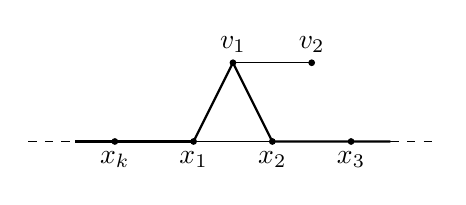
\begin{tikzpicture}
\filldraw[black](0,0)node[below]{$x_1$} circle(1pt);
\draw[very thin](0,0)--(1,0);
\filldraw[black](1,0)node[below]{$x_2$} circle(1pt);
\filldraw[black](-1,0)node[below]{$x_k$} circle(1pt);
\draw[thick](0,0)--(-1.5,0);
\draw[dashed](-2.1,0)--(-1.5,0);
\draw[thin](0.5,1)node[above]{$v_1$}--(1.5,1)node[above]{$v_2$};
\filldraw[black](0.5,1) circle(1pt);
\filldraw[black](1.5,1) circle(1pt);
\draw[thick](0,0)--(0.5,1)--(1,0)--(2.5,0);
\filldraw[black](2,0)node[below]{$x_3$} circle(1pt);
\draw[dashed](2.5,0)--(3.1,0);




\end{tikzpicture}
\end{center}
\end{figure}

\item if $x_2v_2\in E(G)$, then $x_1v_1v_2x_2x_3\cdots x_kx_1$ is a longer cycle, 
\begin{figure}[h]
\begin{center}
\caption{The case $x_2v_2\in E(G)$}
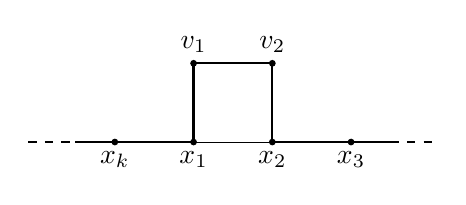
\begin{tikzpicture}
\filldraw[black](0,0)node[below]{$x_1$} circle(1pt);
\draw[very thin](0,0)--(1,0);
\filldraw[black](1,0)node[below]{$x_2$} circle(1pt);
\filldraw[black](-1,0)node[below]{$x_k$} circle(1pt);
\draw[thick](0,0)--(-1.5,0);
\draw[dashed](-2.1,0)--(-1.5,0);
\draw[thick](0,1)node[above]{$v_1$}--(1,1)node[above]{$v_2$};
\filldraw[black](0,1) circle(1pt);
\filldraw[black](1,1) circle(1pt);
\draw[thick](0,0)--(0,1);\draw[thick](1,1)--(1,0)--(2.5,0);
\filldraw[black](2,0)node[below]{$x_3$} circle(1pt);
\draw[dashed](2.5,0)--(3.1,0);


\end{tikzpicture}
\end{center}
\end{figure}
\item if $x_2v_1,x_2v_2\not\in E(G)$, then apply the $2K_2$-free property to $v_1v_2$ and $x_2x_3$, we get either $x_3v_1\in E(G)$ or $x_3v_2\in E(G)$.
\begin{enumerate}
\item if $x_3v_2\in E(G)$, then $C'=x_1v_1v_2x_3\cdots x_kx_1$ is a longer cycle,
\begin{figure}[h]
\begin{center}
\caption{The case $x_3v_2\in E(G)$}
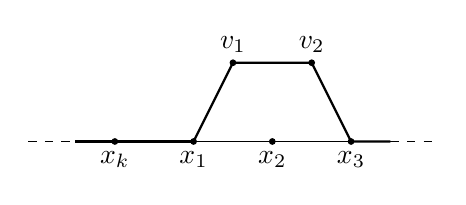
\begin{tikzpicture}
\filldraw[black](0,0)node[below]{$x_1$} circle(1pt);

\filldraw[black](1,0)node[below]{$x_2$} circle(1pt);
\filldraw[black](-1,0)node[below]{$x_k$} circle(1pt);
\draw[thick](0,0)--(-1.5,0);
\draw[dashed](-2.1,0)--(-1.5,0);
\draw[thin](0.5,1)node[above]{$v_1$}--(1.5,1)node[above]{$v_2$};
\filldraw[black](0.5,1) circle(1pt);
\filldraw[black](1.5,1) circle(1pt);
\draw[thick](0,0)--(0.5,1)--(1.5,1)--(2,0)--(2.5,0);
\draw[very thin](0,0)--(2,0);
\filldraw[black](2,0)node[below]{$x_3$} circle(1pt);
\draw[dashed](2.5,0)--(3.1,0);
\end{tikzpicture}
\end{center}
\end{figure}
\item if $x_3v_2\not\in E(G)$, then $x_3v_1\in E(G)$.
\begin{enumerate}
\item if $x_2$ is adjacent to no vertex outside $C$, then we use $C'=x_1v_1x_3\cdots x_kx_1$ to instead $C$. We know that $C$ and $C'$ have the same length, but $C'$ dominates all the edges who are dominated by $C$, and $C'$ also dominates $v_1v_2$, who is not dominated by $C$. So $t$ becomes smaller.

\begin{figure}[h]
\begin{center}
\caption{$x_3v_2\not\in E(G)$, $x_3v_1\in E(G)$, $x_2$ is adjacent to no vertex outside $C$}
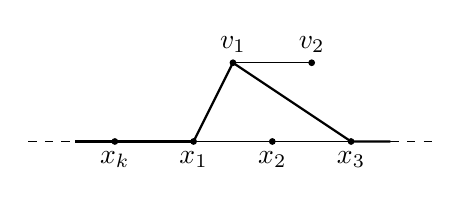
\begin{tikzpicture}
\filldraw[black](0,0)node[below]{$x_1$} circle(1pt);

\filldraw[black](1,0)node[below]{$x_2$} circle(1pt);
\filldraw[black](-1,0)node[below]{$x_k$} circle(1pt);
\draw[thick](0,0)--(-1.5,0);
\draw[dashed](-2.1,0)--(-1.5,0);
\draw[thin](0.5,1)node[above]{$v_1$}--(1.5,1)node[above]{$v_2$};
\filldraw[black](0.5,1) circle(1pt);
\filldraw[black](1.5,1) circle(1pt);
\draw[thick](0,0)--(0.5,1)--(2,0)--(2.5,0);
\draw[very thin](0,0)--(2,0);
\filldraw[black](2,0)node[below]{$x_3$} circle(1pt);
\draw[dashed](2.5,0)--(3.1,0);
\end{tikzpicture}
\end{center}
\end{figure}








\item if $x_2$ is adjacent to some vertices outside $C$, say $z$, for example.

Recall that $x_2$ is adjacent to neither $v_1$ nor $v_2$, then $z$ must be adjacent to either $v_1$ or $v_2$. If $zv_1\in E(G)$, then $C'=x_1v_1zx_2x_3\cdots x_kx_1$ is a longer cycle.



\begin{figure}[h]
\begin{center}
\caption{$x_3v_2\not\in E(G)$, $x_3v_1\in E(G)$, $x_2$ is adjacent to a vertex $z$ outside $C$}
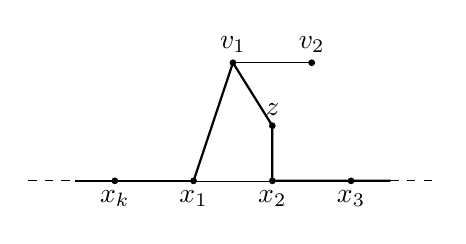
\begin{tikzpicture}
\filldraw[black](0,0)node[below]{$x_1$} circle(1pt);

\filldraw[black](1,0)node[below]{$x_2$} circle(1pt);
\filldraw[black](-1,0)node[below]{$x_k$} circle(1pt);
\draw[thick](0,0)--(-1.5,0);
\draw[dashed](-2.1,0)--(-1.5,0);
\draw[thin](0.5,1.5)node[above]{$v_1$}--(1.5,1.5)node[above]{$v_2$};
\filldraw[black](0.5,1.5) circle(1pt);
\filldraw[black](1.5,1.5) circle(1pt);
\draw[thick](0,0)--(0.5,1.5)--(1,0.7)--(1,0)--(2.5,0);
\draw[very thin](0,0)--(2,0);
\filldraw[black](2,0)node[below]{$x_3$} circle(1pt);
\filldraw[black](1,0.7)node[above]{$z$} circle(1pt);
\draw[dashed](2.5,0)--(3.1,0);
\end{tikzpicture}
\end{center}
\end{figure}





If $zv_2\in E(G)$, then $C'=x_1v_1v_2zx_2x_3\cdots x_kx_1$ is a longer cycle.

\begin{figure}[h]
\begin{center}
\caption{$x_3v_2\not\in E(G)$, $x_3v_1\in E(G)$, $x_2$ is adjacent to a vertex $z$ outside $C$}
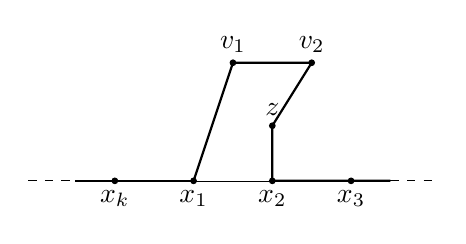
\begin{tikzpicture}
\filldraw[black](0,0)node[below]{$x_1$} circle(1pt);

\filldraw[black](1,0)node[below]{$x_2$} circle(1pt);
\filldraw[black](-1,0)node[below]{$x_k$} circle(1pt);
\draw[thick](0,0)--(-1.5,0);
\draw[dashed](-2.1,0)--(-1.5,0);
\draw[thin](0.5,1.5)node[above]{$v_1$}--(1.5,1.5)node[above]{$v_2$};
\filldraw[black](0.5,1.5) circle(1pt);
\filldraw[black](1.5,1.5) circle(1pt);
\draw[thick](0,0)--(0.5,1.5)--(1.5,1.5)--(1,0.7)--(1,0)--(2.5,0);
\draw[very thin](0,0)--(2,0);
\filldraw[black](2,0)node[below]{$x_3$} circle(1pt);
\filldraw[black](1,0.7)node[above]{$z$} circle(1pt);
\draw[dashed](2.5,0)--(3.1,0);
\end{tikzpicture}
\end{center}
\end{figure}
\end{enumerate}

\end{enumerate}
\end{enumerate}

Repeat the process above. We know the length of a cycle in $G$ is limited, then the process will stop in finite steps. Finally, there will be no edge independent with the cycle from the last step. That is the edge-dominating cycle we want.




\end{proof}








\section{Hamilton prisms of $2K_2$-free graphs}\label{sec55hpo2}

We have already proved, in the last section, that every 1-tough $2K_2$-free graph admits a 2-walk. So, we can expect reasonably that a little higher toughness may guarantee the existence of Hamilton prisms. In this section, we shall show this is true. Specifically, we can prove:
\begin{theorem}[Gao, Pasechnik 2015]\label{mthm21ettohpr}
Suppose $G$ is $2K_2$-free graph, if $G$ is $(1+\epsilon)$-tough for some $\epsilon>0$, then $G$ is prism-Hamiltonian.
\end{theorem}

\subsection{Two special cases}
Before the main part of the proof of Theorem \ref{mthm21ettohpr}, let us look at two special cases.
\subsubsection{$2K_2$-free graph $G$ is a tree}
If $2K_2$-free graph $G$ is a tree, we claim that there are at most two vertices of $G$ with degree larger than 1.
To see this, choose a longest path in $G$, say $u_1u_2\cdots u_w$. If $w\ge5$, by $2K_2$-freeness, there will be a cycle in $G$. Contradiction. Thus $w\le4$. Since this path is a longest one, then no vertex is adjacent to $u_1$ and $u_w$. So, all other vertices in $G$ are adjacent to $u_2$ or $u_{w-1}$ (if they are different). Obviously, all vertices adjacent to $u_2$ and $u_{w-1}$ have degree 1, otherwise, we can get a longer path.

Then by 1-toughness, we see that $G$ is a single edge. Certainly, $G$ is prism-Hamiltonian, here.





\subsubsection{$2K_2$-free graph $G$ is triangle-free}
By Theorem \ref{2k2ftrif1th} in Section \ref{sec511}, every 1-tough triangle-free $2K_2$-free graph $G$ is Hamilotnian, then certainly prism-Hamiltonian. So there is nothing to prove in this case.








\subsection{The proof of Theorem \ref{mthm21ettohpr}}

Now, we only need to take care of the case where $2K_2$-free graph $G$ is not a tree and contains a triangle.
Denote the triangle in $G$ by $XX'X''$. If the 3-cycle $XX'X''$ is edge-dominating, then we have finished our proof. If not, there is an edge $u_1u_2$, with no endpoint on the 3-cycle. Then by $2K_2$-freeness, $u_1$ and $u_2$ have at least two neighbors, say $X$ and $X'$, on the cycle.

\paragraph{If $u_1X\in E(G)$ and $u_2X'\in E(G)$,} (the case $u_2X'\in E(G)$ and $u_1X'\in E(G)$ is similar), we get a 5-cycle $XX''X'u_2u_1X$ in $G$.

\paragraph{If $u_1X,u_1X'\in E(G)$,}(the case $u_2X,u_2X'\in E(G)$ is similar), we get a 4-cycle $XX''X'u_1X$ with a diagnoal $XX'$. If this 4-cycle is edge-dominating, we have done. Otherwise, there is an edge, say $u_3u_4$ with no endpoint on the 4-cycle. Then $u_3$ and $u_4$ have at least two neighbors in $X$, $X'$ and $X''$. By the $2K_2$-free arguing on $u_1u_2$ and $u_3u_4$, we can always get a cycle with length at least 5, and containing $X$, $X'$ and $X''$ successively (the order may be changed).


\paragraph{Now, we shall show that whenever $G$ has a cycle $C=x_1x_2\cdots x_kx_1$ of length $k\ge5$, and $X$, $X'$ and $X''$ are three successive vertices on $C$, then one of the following statements is true.}
\begin{enumerate}
\item $C$ is edge-dominating.
\item There is a longer cycle $C'$ in $G$ also contains $X$, $X'$ and $X''$ successively.
\item There is a cycle $C'$ with length $k$, containing $X$, $X'$ and $X''$ successively, but dominates more edges than $C$.
\end{enumerate}

Suppose $C$ is not edge-dominating. Then there is an edge, namely $v_1v_2\in E(G)$ with no endpoint on $C$. Assume $X'XX''$ is the order of these three vertices on $C$, by $2K_2$-free arguing, $v_1$ and $v_2$ have at least one neighbor in $\{X',X''\}$. We assume $v_1X'\in E(G)$. Then we label the vertices in $C$ in the following way.

$X'$ is labeled by $x_1$. The neighbor of $x_1$ (on $C$), who is not $X$, is labeled by $x_2$. Other vertices on $C$ is labeled successively. Then, certainly, $X''$ is labeled by $x_{k-1}$ and $X$ is labeled by $x_k$. See the following picture (Figure \ref{labelcycle}).

\begin{figure}[h]
\begin{center}
\caption{The cycle $C$ of length $k$}\label{labelcycle}
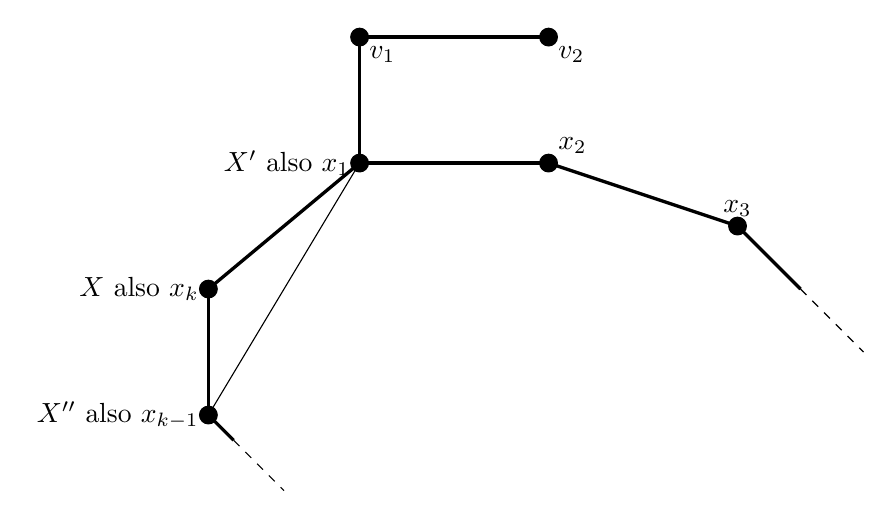
\begin{tikzpicture}[scale=1.6]


\filldraw[black](0,0)node[left]{$X'$ also $x_1$} circle(2pt);
\filldraw[black](1.5,0)node[above right]{ $x_2$} circle(2pt);
\filldraw[black](3,-0.5)node[above]{ $x_3$} circle(2pt);
\draw[very thick](0,0)--(1.5,0);
\draw[very thick](3,-0.5)--(1.5,0);
\draw[very thick](3,-0.5)--(3.5,-1);
\draw[dashed](3.5,-1)--(4,-1.5);

\filldraw[black](-1.2,-1)node[left]{$X$ also $x_k$} circle(2pt);
\draw[very thick](0,0)--(-1.2,-1);

\filldraw[black](-1.2,-2)node[left]{$X''$ also $x_{k-1}$} circle(2pt);
\draw[very thick](-1.2,-2)--(-1.2,-1);
\draw[very thick](-1.2,-2)--(-1,-2.2);
\draw[dashed](-1,-2.2)--(-0.6,-2.6);

\filldraw[black](0,1)node[below right]{ $v_1$} circle(2pt);
\draw[very thick](0,1)--(1.5,1);
\filldraw[black](1.5,1)node[below right]{ $v_2$} circle(2pt);
\draw[very thick](0,1)--(0,0);
\draw[thin](0,0)--(-1.2,-2);



\end{tikzpicture}
\end{center}
\end{figure}

Note that the operation (in the proof of the first part of Theorem \ref{cothm2kwin2kpol}) of enlarging the cycle $C$ to $C'$ has nothing to do with the edges $x_{k-1}x_k$ and $x_kx_1$ when $k\ge5$. Thus the three vertices $X''$, $X$ and $X'$ are always successive on the cycle in our process. Then we can finally find the edge-dominating cycle contains three vertices of a triangle successively.


By Theorem \ref{edhctohprthlm}, we have finished our proof.
\qed






\section{A generalization: $3K_2$-free graphs}\label{sec553k2}
In this section, let us look at a generalization of $2K_2$-free graphs. Similar to the definition of $2K_2$-free graphs, a {\em $3K_2$-free graph} is a graph does not contain any copy of $3K_2$ as induced subgraph.

\subsection{The structure of $3K_2$-free graph}
Suppose $H$ is a $3K_2$-free graph. If $H$ is also $2K_2$-free, we have already known a lot of information about is, so in this section, we assume $H$ contains at least one copy of $2K_2$ as an induced subgraph. Choose a $2K_2$ from $H$, and denote its two edges by $e_1=v_1v_2$ and $e_2=v_3v_4$. Define a function $f_{H,U}(v)$ for $v\in V(H)$ in the following way.
\begin{enumerate}
\item $f_{H,U}(v)=0$, if $v\in U=\{v_1,v_2,v_3,v_4\}$.
\item $f_{H,U}(v)=1$, if $v$ is not in $\{v_1,v_2,v_3,v_4\}$, but $v$ is adjacent to some of them.
\item $f_{H,U}(v)=2$, otherwise.
\end{enumerate}

By $3K_2$-freeness, the following two statements are easy to prove.
\begin{theorem}
The subset of vertices $\{v\in V(H)|f_{H,U}(v)=2\}$ is an independent set.
\end{theorem}

\begin{theorem}
Each vertex in $\{v|f_{H,U}(v)=2\}$ is adjacent to some vertices in $\{v|f_{H,U}(v)=1\}$.
\end{theorem}

Here (see Figure \ref{pic3k2f561}), we draw an example of $3K_2$-free graph, with a function $f_{H,U}$. The vertices in $\{v|f_{H,U}(v)=1\}$ are denoted by $u_i$ and the vertices in $\{v|f_{H,U}(v)=2\}$ are denoted by $w_i$.

\begin{figure}[h]
\begin{center}
\caption{An example of $3K_2$-free graph}\label{pic3k2f561}
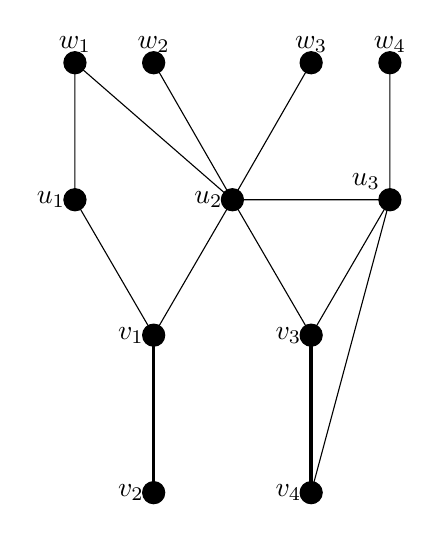
\begin{tikzpicture}[scale=2]

\filldraw[black](0,0)node[left]{$v_1$} circle(2pt);
\filldraw[black](0,-1)node[left]{$v_2$} circle(2pt);
\filldraw[black](1,0)node[left]{$v_3$} circle(2pt);
\filldraw[black](1,-1)node[left]{$v_4$} circle(2pt);
\filldraw[black](0.5,0.86)node[left]{$u_2$} circle(2pt);
\filldraw[black](-0.5,0.86)node[left]{$u_1$} circle(2pt);
\filldraw[black](1.5,0.86)node[above left]{$u_3$} circle(2pt);
\filldraw[black](-0.5,1.73)node[above]{$w_1$} circle(2pt);
\filldraw[black](0,1.73)node[above]{$w_2$} circle(2pt);
\filldraw[black](1,1.73)node[above]{$w_3$} circle(2pt);
\filldraw[black](1.5,1.73)node[above]{$w_4$} circle(2pt);
\draw(-0.5,1.73)--(-0.5,0.86)--(0,0)--(0.5,0.86)--(0,1.73);
\draw[very thick](0,0)--(0,-1);
\draw[very thick](1,0)--(1,-1);
\draw(1.5,1.73)--(1.5,0.86)--(1,0)--(0.5,0.86)--(-0.5,1.73);
\draw(1,1.73)--(0.5,0.86)--(1.5,0.86)--(1,-1);




\end{tikzpicture}
\end{center}
\end{figure}




\newpage

\subsection{2-walks in $3K_2$-free graphs}
Now, let us look at the existence of 2-walks in $3K_2$-free graphs.
In fact it is easy to prove the following result.

\begin{theorem}\label{thm3k2f1t2w}
Every 1-tough $3K_2$-free graph admits a 2-walk.
\end{theorem}

\begin{proof}
To prove this theorem, we only need to combine Corollary \ref{co32c3kfed} and Theorem \ref{mthm1}, and note that every 1-tough graph is 2-connected.
\end{proof}





\section{Some open problems for further research}

In the end of this chapter, we list several conjectures, which may be true,  relevant to this topic.

\begin{conjecture}
Every 2-tough $2K_2$-free graph on at least 3 vertices is Hamiltonian.
\end{conjecture}

\begin{conjecture}
Every $3/2$-tough $2K_2$-free graph on at least 3 vertices admits a 2-trail, i.e. a 2-walk with each edge appearing in the walk at most once.
\end{conjecture}

\begin{conjecture}
Every 1-tough $2K_2$-free graph is prism-Hamiltonian.
\end{conjecture}


\begin{conjecture}
Every 1-tough $3K_2$-free graph is prism-Hamiltonian.
\end{conjecture}








\chapter{Conclusions}
In this work, we focus on a serious of generalizations of Hamilton cycles, $k$-trees and $k$-walks., and their existence under toughness conditions.
For Hamiltonicity the most important conjecture, Chv{\'a}tal's Conjecture is still open now. For $k$-walks, we have already known that $\frac{1}{k-2}$-toughness is sufficient for the existence of $k$-walk, but we wish we can reduce the requirement to $\frac{1}{k-1}$-toughness, this conjecture is open in general, as Jackson-Wormald's Conjecture. 

However, we proved that for $2K_2$-free graphs, this conjecture is true. In our research, we investigated the structure of $2K_2$-free graphs, for example, the dominating-weakly-dominating-clique sequence of a $2K_2$-free graph and the relation between $2K_2$-free graphs and split graphs.

In our work, we show that the existence of edge-dominating cycles is a sufficient (possibly not necessary) condition for the existence of $k$-walks under $\frac{1}{k-1}$-toughness. In 1983, Veldman pointed out the existence of edge-dominating cycles for many kinds of graphs, including $2K_2$-free graphs. However, Veldman did not tell us how to find the edge-dominating cycles out. In our work, we found edge-dominating cycles for $2K_2$-free graphs by a constructive method, and also proved that  this method can be finished in time polynomial to the number of vertices of the graphs.

Furthermore, we note that being prism-Hamiltonian is also a good measure on how close a graph close to being Hamiltonian. In fact, being prism-Hamiltonian is stronger than admiting a 2-walk, but weaker than being traceable. In our research, we proved that if a $(1+\epsilon)$-tough graph admits an edge-dominating cycle, with a triangle on proper position on the edge-dominating cycle, then it is prism-Hamiltonian. After more elaborate analysis on the edge-dominating cycles of $2K_2$-free graphs, we obtained that the edge-dominating cycle of $2K_2$-free graphs have the triangles meeting our requirement. Therefore, we proved that every $(1+\epsilon)$-tough $2K_2$-free graph is prism-Hamiltonian.

Finally, we list several conjectures, which are possibly true, on the existence of Hamilton cycles, Hamilton trails and Hamilton prisms.

















\bibliography{treftough}

\bibliographystyle{plain}






\end{document}
